\documentclass[man,12pt,floatsintext]{apa7}
% - stu: this sets the `document mode' as the "student paper" version. Other options are jou (journal), man (manuscript, for journal submission), and doc (a plain document)
% --- The student setting includes things like 'duedate', 'course', and 'professor' on the title page. If these aren't wanted/needed, use the 'man' setting. It also defaults to including the tables and figures at the end of the document. This can be changed by including the 'floatsintext' option, as I have for you. If the instructor wants those at the end, remove that from the square brackets.
% --- The manuscript setting is roughly what you would use to submit to a journal, so uses 'date' instead of 'duedate', and doesn't include the 'course' or 'professor' info. As with 'stu', it defaults to putting the tables and figures at the end rather than in text. The same option will bump those images in text.
% --- Journal ('jou') outputs something similar to a common journal format - double columned text and figurs in place. This can be fun, especially if you are sumbitting this as a writing sample in applications.
% --- Document ('doc') outputs single columned, single spaced text with figures in place. Another option for producing a more polished looking document as a writing sample.
% - 12pt: sets the font size to 12pt. Other options are 10pt or 11pt
% - floatsintext: makes it so tables and figures will appear in text rather than at the end. Unforunately, not having this option set breaks the whole document, and I haven't been able to figure out why. IT's GREAT WHEN THINGS WORK LIKE THEY'RE SUPPOSED TO.
\usepackage[american]{babel}
\usepackage{csquotes}
\usepackage[style=apa,sortcites=true,sorting=nyt,backend=biber]{biblatex}
\DeclareLanguageMapping{american}{american-apa}
\addbibresource{bibliography.bib}
\usepackage[T1]{fontenc}
\usepackage{mathptmx}
% --- Math/fig/table helpers (safe with apa7) ---
\usepackage{amsmath,amssymb,bm}
\usepackage{graphicx}
\usepackage{booktabs}
\usepackage{siunitx}
\usepackage{hyperref}
\usepackage{enumitem}
\usepackage{subcaption}
% for referencing sections
\usepackage{nameref}
% for table
\usepackage{booktabs}
\usepackage{threeparttable}
\usepackage{tabularx}
\usepackage{setspace}
\usepackage{siunitx}
\usepackage{array}
\usepackage{multirow}
\usepackage[table]{xcolor}
\definecolor{rulegray}{gray}{0.82}
\definecolor{bandgray}{gray}{0.97}
\newcolumntype{L}[1]{>{\raggedright\arraybackslash}m{#1}}
\newcolumntype{C}[1]{>{\centering\arraybackslash}m{#1}}
% Title page stuff _____________________
\title{When Context Looks Like Coupling: A Slow--Fast Theory of Psychological Dynamics}
\shorttitle{Slow--Fast Psychological Dynamics}
\author{%
Kyuri Park\textsuperscript{*1},
Denny Borsboom\textsuperscript{3},
Mike Lees\textsuperscript{1,2},
Lourens Waldorp\textsuperscript{3},
Johan Bollen\textsuperscript{1},
Vítor V.\ Vasconcelos\textsuperscript{1,2}
}
\affiliation{%
\textsuperscript{1} University of Amsterdam\mbox{,} Informatics Institute\mbox{,} Computational Science Lab\\
\textsuperscript{2} University of Amsterdam\mbox{,} Institute for Advanced Study\\
\textsuperscript{3} University of Amsterdam\mbox{,} Department of Psychology
}
\authornote{%
\textbf{Author contact information.}
Kyuri Park (\href{mailto:k.park@uva.nl}{k.park@uva.nl});
Vítor V.\ Vasconcelos (\href{mailto:v.v.vasconcelos@uva.nl}{v.v.vasconcelos@uva.nl});
Mike Lees (\href{mailto:m.h.lees@uva.nl}{m.h.lees@uva.nl});
Denny Borsboom (\href{mailto:d.borsboom@uva.nl}{d.borsboom@uva.nl});
Lourens Waldorp (\href{mailto:l.j.waldorp@uva.nl}{l.j.waldorp@uva.nl});
Johan Bollen (\href{mailto:j.bollen@uva.nl}{j.bollen@uva.nl}).\\[0.5em]
\textbf{Affiliation addresses.}\\
\textsuperscript{1} University of Amsterdam, Informatics Institute, Computational Science Lab,
PO Box 94323, 1090 GH Amsterdam, The Netherlands.\\
\textsuperscript{2} University of Amsterdam, Institute for Advanced Study,
Oude Turfmarkt 147, 1012 GC Amsterdam, The Netherlands.\\
\textsuperscript{3} University of Amsterdam, Department of Psychology,
Nieuwe Achtergracht 129, 1018 WS Amsterdam, The Netherlands.\\[0.5em]
\textbf{Correspondence.}
*Correspondence concerning this article should be addressed to Kyuri Park.
}
% for Psychological Review:
\abstract{
\begingroup
\setstretch{1.3}\selectfont
Many psychological states change quickly, but the conditions that make them likely often change
slowly. Symptoms, affect, attention, motivation, and interpersonal behavior can fluctuate over
short timescales, whereas stress exposure, social support, financial strain, biological
vulnerability, developmental history, and relational context often change more gradually. This
difference in timescale matters because slow conditions can shape the activation of fast states.
When those conditions are not represented in a model, their effects may be misread as stronger
relations among the fast states themselves.
We develop this argument through the case of psychopathology symptom networks. Between-group
differences in estimated symptom networks are often interpreted as evidence that
symptom--symptom coupling differs across populations. We ask when similar between-group patterns
can arise even when symptom--symptom coupling is held fixed. To address this question, we develop
a coupled slow--fast computational model in which symptoms evolve on a fast timescale, while a
slower contextual process shifts the ease with which symptoms become active.
In the model, symptoms are binary states that reinforce one another through a shared mean-field
interaction. Depending on the strength of this reinforcement, the symptom system has either a
single stable symptom level or two alternative stable levels, corresponding to low- and
high-symptom states. The slow state shifts symptom activation and is itself affected by sustained
symptom elevation, creating feedback between fast symptom dynamics and slower contextual change.
Simulations show that pronounced between-group differences can emerge without any change in
symptom--symptom coupling. Depending on the slow-state baseline, feedback, and acute stressors,
the model produces stable between-group separation, temporary stress-related worsening, or abrupt
and persistent transitions into high-symptom states. A network-estimation check further shows that
omitting the slow context can inflate estimated global strength and impair recovery of the true
coupling matrix, whereas including the slow context substantially reduces this distortion.
These results suggest that differences in estimated symptom networks should not be interpreted
automatically as differences in symptom--symptom coupling. More broadly, they point to a
slow--fast principle for psychological theory: fast-changing states unfold within slower-moving
conditions that shape what responses become likely, stable, or difficult to escape.
\par
\endgroup
}
% \abstract{
% \begingroup
% \setstretch{1.3}\selectfont
% Between-group differences in psychopathology symptom networks are often interpreted as evidence that symptom--symptom coupling differs across populations. This paper asks under what conditions similar between-group patterns can arise even when symptom--symptom coupling is held fixed across groups. To address this question, we develop a coupled slow--fast computational model in which symptoms evolve on a fast timescale, while a slower contextual process shifts overall symptom activation over time.
% The fast layer represents symptoms as binary states that reinforce one another through a shared mean-field interaction. Depending on the strength of this reinforcement, the symptom system has either a single stable symptom level or two alternative stable levels, corresponding to low- and high-symptom states. The slow state shifts the overall ease with which symptoms become active and is itself affected by sustained symptom elevation, creating feedback between fast symptom dynamics and slower contextual change. We analyze the resulting equilibrium structure to identify when slow threshold shifts should produce gradual group separation, abrupt tipping, or path-dependent switching.
% Simulation experiments show that pronounced between-group differences can emerge without any change in symptom--symptom coupling. Depending on the slow-state baseline, feedback, and acute stressors, the model produces stable between-group separation, temporary stress-related worsening, or abrupt and persistent transitions into high-symptom states. A compact network-estimation check further shows that omitting the slow context can inflate estimated global strength and impair recovery of the true coupling matrix, whereas including the slow context substantially reduces this distortion.
% These results matter for interpreting psychological networks: apparent connectivity may partly reflect unmodeled slow contextual variation rather than altered symptom--symptom coupling. More broadly, the model captures a general slow--fast principle in psychology: fast-changing states such as affect, motivation, attention, executive control, and interpersonal behavior unfold within slower-moving social, relational, economic, and biological conditions that shape what responses become likely, stable, or difficult to escape. Slow--fast coupling therefore offers a general framework for modeling psychological systems across interacting timescales.
% \par
% \endgroup
% }
\keywords{slow--fast systems; psychological dynamics; timescale separation; symptom networks; computational modeling}
\begin{document}
\maketitle % This tells LaTeX to make the title page
% ==================================================================
% Introduction
% ==================================================================
%\section{Introduction}
Network approaches to psychopathology start from a simple observation: symptoms do not merely co-occur; they can influence one another. Insomnia can lead to fatigue, fatigue can reduce concentration, concentration problems can interfere with work, and these difficulties can in turn worsen mood or increase feelings of failure. In this view, symptoms are not passive indicators of an underlying disorder, but components of a system whose dynamics can become self-sustaining \parencite{borsboom2017network, robinaugh2020network}. When symptom--symptom relations are strong enough, activation may persist after the original trigger has disappeared, and the system may shift into a stable high-symptom state \parencite{van2014critical}.
At the same time, symptoms do not arise in isolation from the broader conditions of a person's life. Stressful events, social isolation, financial insecurity, sleep disruption, inflammation, or other contextual and biological processes can make symptoms easier or harder to (de) activate. In network terms, these influences belong to the external field of the symptom system: they are not themselves symptoms in the network, but they change the conditions under which symptoms become active. This distinction matters because the same symptom network may behave very differently depending on the surrounding field. A weak perturbation may fade when symptoms are difficult to activate, whereas a similar perturbation may trigger persistent symptom activation when the background conditions have shifted the system closer to a transition point.
This raises a problem for a common empirical practice in psychopathology network research. Researchers often estimate symptom networks separately across groups that differ in illness course, treatment stage, or exposure history, such as persistent versus remitted depression, admission versus discharge samples, or trauma reporters versus non-reporters \parencite[e.g.,][]{van2015association, beard2016network, peel2021comparison}. These studies typically compare global strength, specific edge weights, or centrality, often using network-comparison procedures \parencite{van2023comparing, haslbeck2022estimating}. A natural interpretation is that differences in estimated edges reflect differences in symptom--symptom coupling: one group appears to have a more strongly connected, more fragile, or differently organized symptom system than another. But this interpretation is not forced by the data.
The reason is already visible in Ising-type models, where symptom activation depends on two ingredients: how strongly symptoms reinforce one another, and how easily symptoms become active in the first place \parencite{ising1925beitrag, brout1959statistical, stanley1971phase, goldenfeld2018lectures}. Network psychometrics has adapted this logic to binary symptom data by representing symptoms as interacting variables with both interaction parameters and threshold parameters \parencite{van2014new, marsman2018introduction}; related network accounts of psychopathology have also used Ising-style reasoning to describe how symptoms may reinforce one another \parencite{cramer2010comorbidity}. Stronger symptom--symptom reinforcement can make high-symptom states more likely, but this effect depends on the baseline ease with which symptoms are activated. In Ising-type models, this baseline activation tendency is captured by the external field, or threshold regime. Therefore, between-group differences in estimated symptom networks may arise not only because coupling differs across groups, but also because groups differ in their threshold regimes while coupling remains fixed \parencite{<our-perspective-paper>}.
The difference between these explanations is not merely technical. If an estimated edge difference is interpreted as a coupling difference, one may conclude that the groups differ in their mechanisms of symptom reinforcement, their most central symptoms, or their most relevant intervention targets. Under a threshold-shift account, the same empirical pattern could instead indicate that one group is exposed to higher slow-contextual load, is closer to a transition boundary, or is already on a different stable branch of the same underlying system. Clinically, these explanations point to different targets. A coupling-based interpretation suggests intervening on symptom--symptom relations or highly central symptoms. A threshold/external-field interpretation points instead to the slower contextual conditions that make symptoms easier to activate or that place individuals near tipping points. Thus, the identification problem also implies a knowledge gap: existing between-group network differences do not by themselves tell us whether groups differ in symptom--symptom coupling, symptom thresholds/external fields, proximity to a transition boundary, or some combination of these.
Several lines of work speak to parts of this problem. Critical-transition approaches in psychopathology have shown how nonlinear symptom systems can display tipping points, hysteresis, and early warning signals \parencite{van2014critical, scheffer2009early, helmich2021early}. Network-psychometric work has formalized the role of thresholds and interactions in Ising models for binary symptom data \parencite{van2014new, marsman2018introduction}. Group-comparison and moderation approaches provide tools for testing whether estimated thresholds or interactions differ across groups \parencite{van2023comparing, haslbeck2022estimating}. Finally, \textcite{lunansky2020personality} introduced an explicitly slow--fast perspective by linking slowly evolving personality and resilience processes to faster psychopathology networks. What remains less clear is how a slowly changing contextual field affects the interpretation of estimated symptom networks, especially when that context is not measured or not included in the network model.
This problem is closely related to existing equivalence results in network psychometrics. Prior work has shown that associations among binary symptoms can often be represented in more than one way: as direct symptom--symptom interactions, as dependence induced by shared latent or common causes, or as item-response structure \parencite{kruis2016three, marsman2018introduction, van2021latent}. These results imply that observed symptom associations do not uniquely identify symptom--symptom coupling. The present paper takes this ambiguity as a starting point. Its contribution is to ask how the ambiguity changes when the shared contextual influence is not static, but unfolds over a slower timescale and is not always included in symptom-network estimation.
Related work on the inverse problem for Ising-type models makes a similar point from a statistical perspective. A large methodological literature asks when interaction parameters in binary graphical models can be recovered from multivariate data. For Ising models, nodewise \(\ell_1\) regularized logistic regression provides one foundational approach to graph selection under high-dimensional consistency conditions \parencite{ravikumar2010high}. More recent work extends this kind of pseudo-likelihood framework to models that include both Ising-type pairwise interactions and covariate-dependent external fields \parencite{mukherjee2024logistic}. These results are methodologically adjacent to the present paper rather than its main contribution: here we use a known data-generating system to ask how omitting a slow contextual input changes what a standard conditional estimator recovers. Conversely, work on reconstructability in dynamical networks shows that pairwise statistical dependence need not recover direct interactions when common-cause, relay, or topological effects contribute to observed associations, although weak-coupling regimes can improve reconstructability \parencite{lunsmann2017transition}. Together, these lines of work reinforce the distinction between direct coupling and association induced by measured or unmeasured contextual structure.
The present paper addresses this problem with a slow--fast computational model. The fast layer represents psychological symptoms that activate and deactivate over short timescales under fixed symptom--symptom coupling. The slow layer represents a contextual state that changes more gradually and shifts the ease with which symptoms become active. We use the model as a known data-generating system: the underlying symptom--symptom coupling is held fixed, while the slow context differs across groups and changes over time.
This setup allows us to ask what an estimated symptom network recovers when symptoms unfold within an unmodeled slow context. We first use the mean-field model to characterize how slow threshold shifts can produce gradual separation, abrupt tipping, and path-dependent switching under fixed reinforcement. We then add a compact network-estimation check in which data are generated with the same symptom--symptom coupling across groups but different slow-context regimes. In doing so, the paper reframes between-group network differences as a dynamic identification problem: the same symptom system may look like a different network when it is observed under different slow-contextual conditions.
% ==========================================================
% Model
% ==========================================================
\section{Model}\label{sec:model}
\subsection{Conceptual overview}
Group differences in symptom networks need not always reflect differences in symptom--symptom coupling. They may also arise because groups differ in the conditions under which symptoms become easy or difficult to activate. The model presented here formalizes this idea by distinguishing two timescales.
On the fast timescale, symptoms switch between inactive and active states. These fluctuations are meant to capture the short-term dynamics of symptom activation: symptoms may appear, disappear, and reinforce one another. On the slow timescale, a broader background state changes more gradually. This slow state may represent chronic stress, contextual pressure, precarity, biological vulnerability, or any other slowly evolving condition that changes the ease with which symptoms become active.
The key assumption is that these two timescales are coupled. The slow state affects the symptom system by shifting its overall activation tendency. At the same time, sustained symptom elevation can feed back into the slow state: prolonged symptoms may worsen social, relational, occupational, or biological conditions, which in turn make symptoms easier to activate. Acute stressful events can also be added as an extension, allowing the same framework to distinguish gradual contextual change from abrupt perturbations. Thus, the core model contains fast symptom dynamics, slow contextual dynamics, and coupling between them. Figure~\ref{fig:slow-fast-illust} provides a schematic overview of this multiscale coupling.
\begin{figure}[htbp]
  \centering
  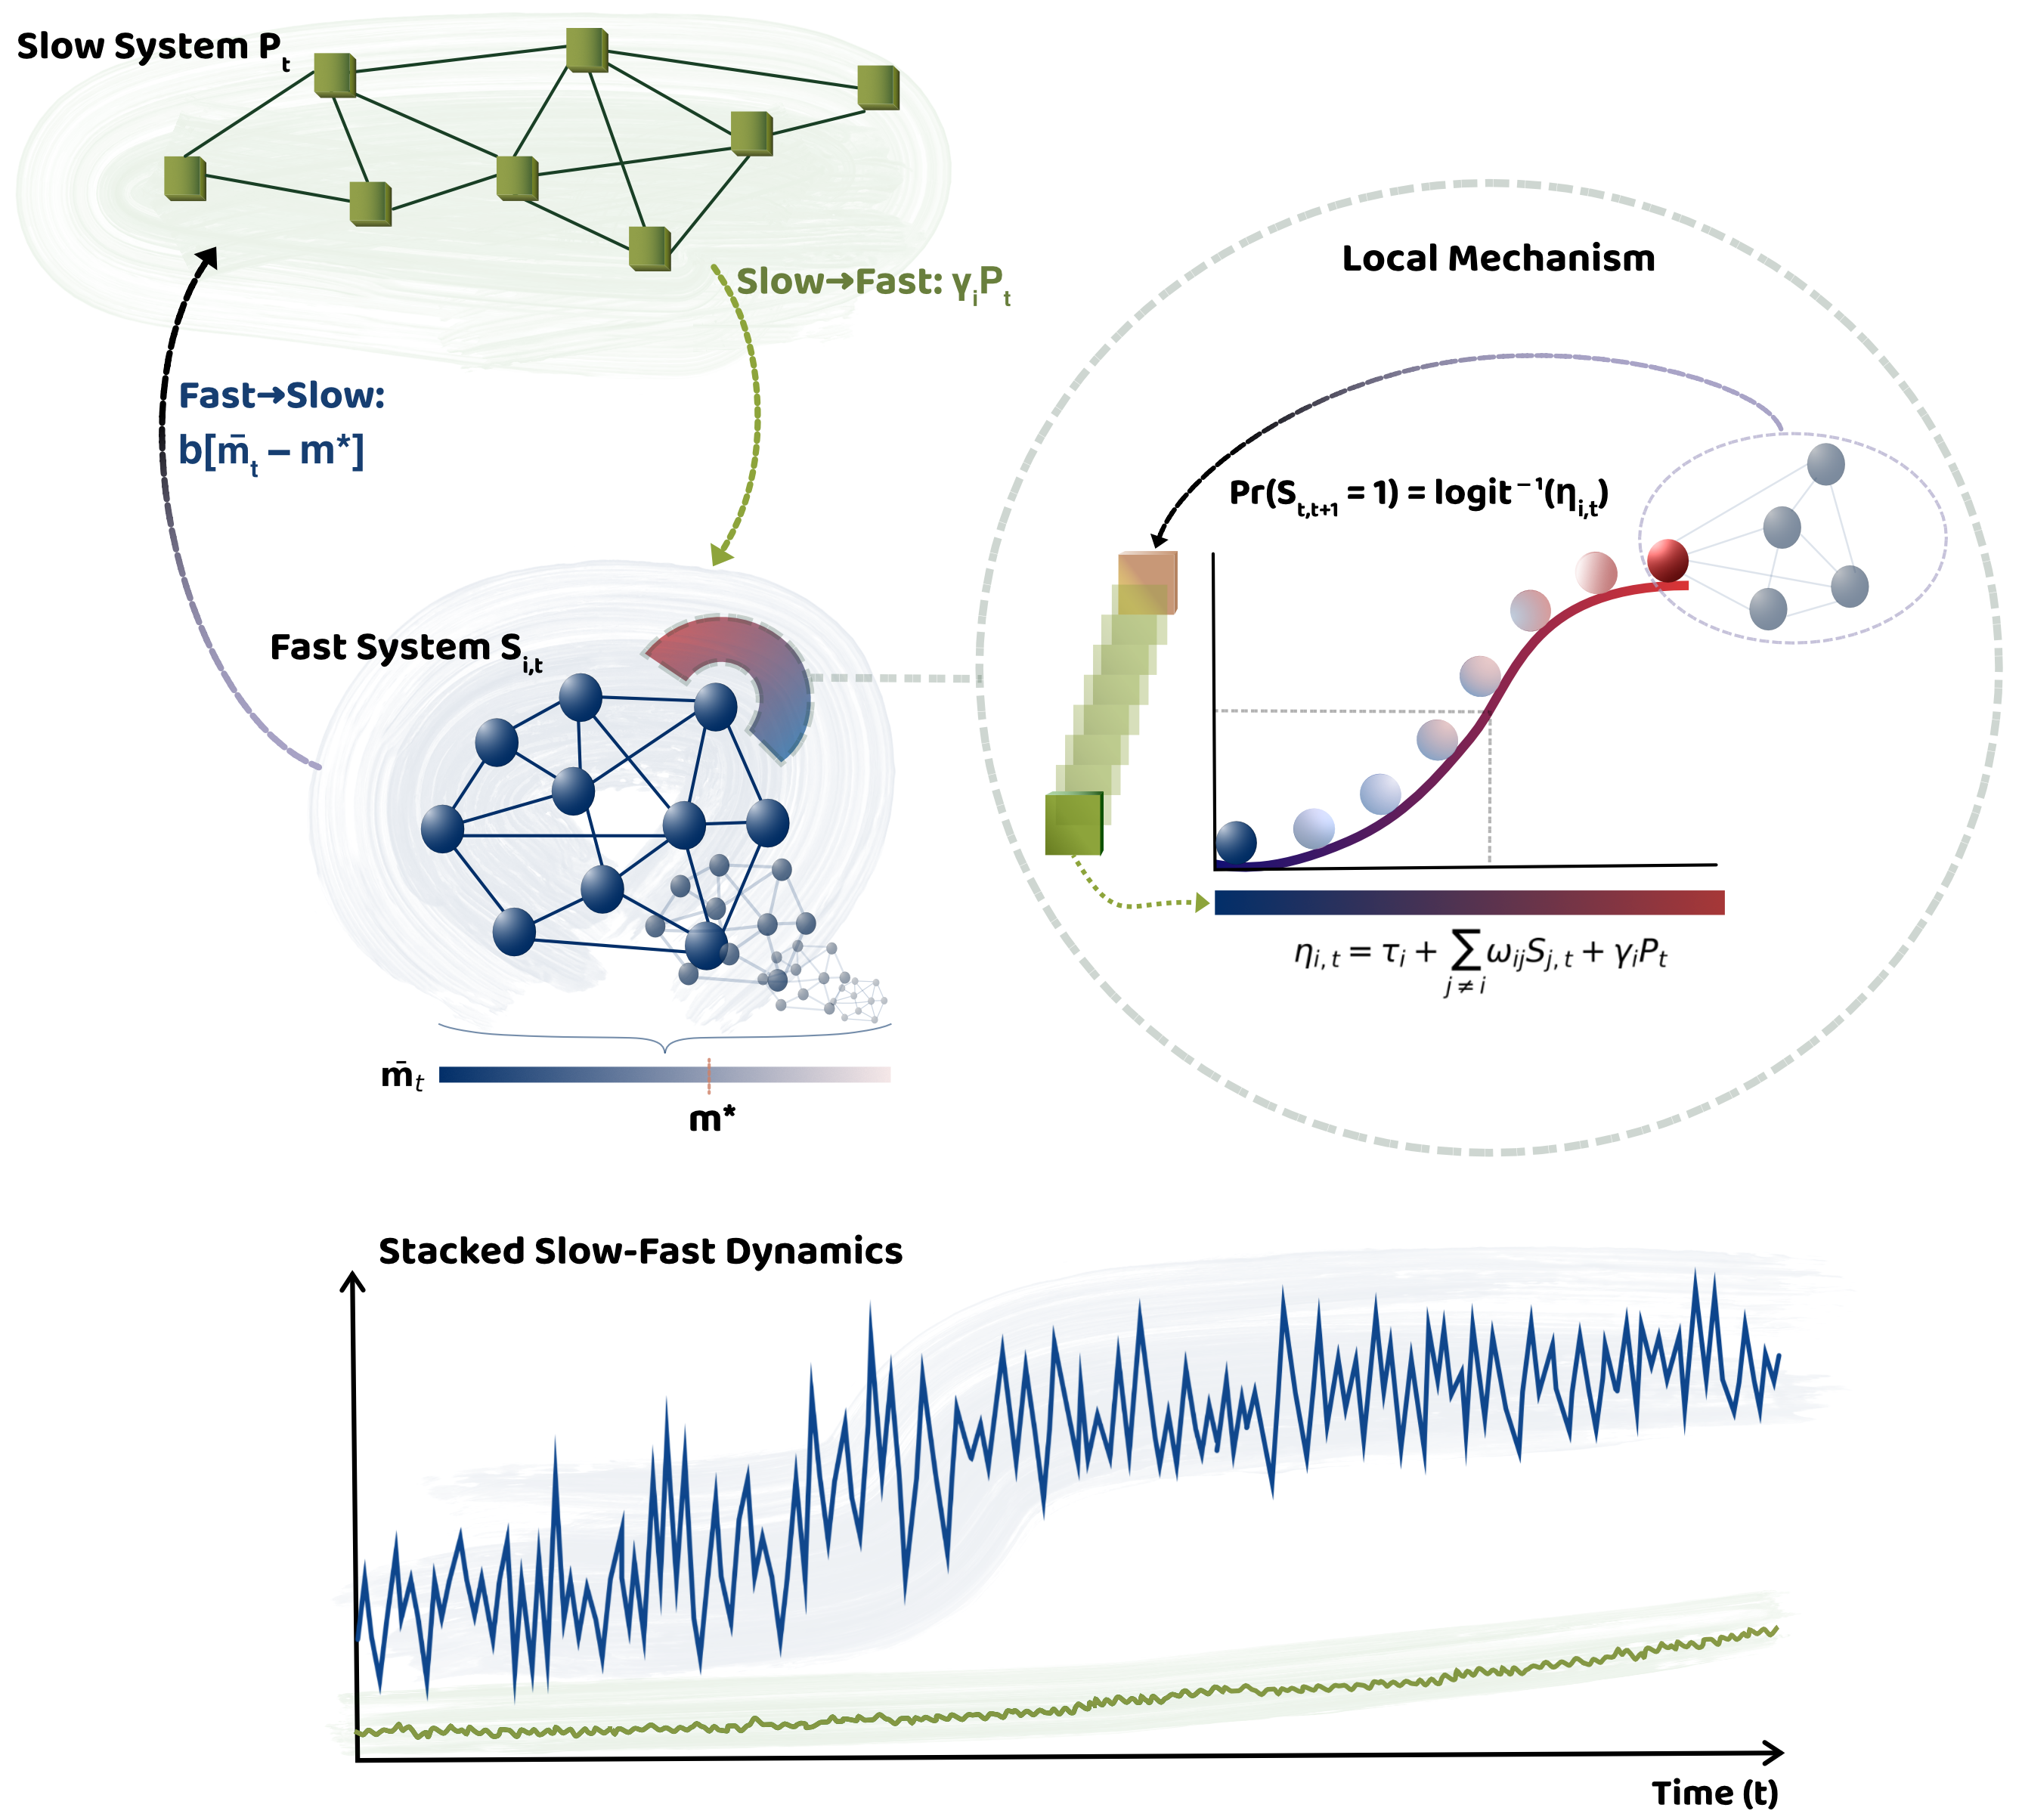
\includegraphics[width=\linewidth]{figs/slow-fast-model-illustration_v2.png}
  \caption{\textbf{Conceptual schematic of the coupled slow--fast model.}
  The fast system (blue network) consists of binary symptoms updated on a fast timescale and summarized by the mean symptom level \(m_t\). The slow system (green) is represented by the scalar slow state \(P_t\), which evolves on a slower timescale. Coupling is bidirectional. \textbf{Slow \(\rightarrow\) fast} (green dashed arrow): the slow state enters the fast-layer input as an additive term \(\gamma P_t\), shifting the net input \(H_t\) and thereby changing symptom activation probabilities (local mechanism inset). \textbf{Fast \(\rightarrow\) slow} (blue dashed arrow): the slow-state drift depends not on the instantaneous symptom level \(m_t\), but on a smoothed symptom signal \(m_{\mathrm{slow},t}\) that retains memory of recent symptom activation. In the schematic, faded copies of the fast network indicate past symptom states whose influence decays over time, while the bar labeled \(m_{\mathrm{slow},t}\) represents their weighted accumulation. This signal enters the slow dynamics through \(b(m_{\mathrm{slow},t}-m^\star)\), pushing \(P_t\) upward when sustained symptom elevation is high and downward when it is low relative to \(m^\star\). The bottom panel illustrates typical stacked dynamics: \(m_t\) fluctuates rapidly while \(P_t\) drifts slowly, with coupling allowing gradual changes in the slow state, and, when included, discrete shocks, to produce large changes in symptom level when the system is near a transition boundary.}
  \label{fig:slow-fast-illust}
\end{figure}
At the fast timescale, the symptom layer is summarized by the mean symptom level \(m_t\), the fraction of symptoms that are active at time \(t\). At the slow timescale, the scalar state \(P_t\) tracks the background condition that shifts symptom activation. The slow-to-fast pathway means that changes in \(P_t\) alter the effective input to the symptom system. The fast-to-slow pathway means that the slow state responds not to every momentary symptom fluctuation, but to a smoothed symptom signal \(m_{\mathrm{slow},t}\), so that persistent symptom elevation matters more than brief spikes. Table~\ref{tab:model-notation} summarizes the main symbols used in the model.
\definecolor{bandgray}{gray}{0.97}
\definecolor{rulegray}{gray}{0.80}
\begin{table}[htbp]
\centering
\caption{Main symbols used in the slow--fast model, organized by layer.}
\label{tab:model-notation}
\setlength{\extrarowheight}{2pt}
\renewcommand{\arraystretch}{1.08}
\begin{tabularx}{\linewidth}{@{} l l X @{}}
\arrayrulecolor{black}\toprule
Symbol & Name & Meaning \\
\midrule
\rowcolor{bandgray}
\multicolumn{3}{c}{\textit{Fast layer}} \\
\(N\) & Number of symptoms & Total number of binary symptoms in the fast layer \\
\(S_{i,t}\) & Symptom state & Binary state of symptom \(i\) at time \(t\); realized value \(s_{i,t}\in\{0,1\}\) \\
\(m_t\) & Mean symptom level & Fraction of symptoms that are active at slow time step \(t\) \\
\(J\) & Interaction strength & How strongly symptoms reinforce one another \\
\(h\) & Baseline intercept & Common baseline tendency toward symptom activation \\
\(\gamma\) & Slow-state effect & How strongly the slow state \(P_t\) shifts symptom activation \\
\(\beta\) & Response sensitivity & How sensitively symptom updates respond to the input \\
\(H(m,p_t)\) & Net input & Net input driving symptom activation at mean symptom level \(m\) and slow state \(p_t\) \\
\arrayrulecolor{rulegray}\specialrule{0.4pt}{3pt}{0pt}
\rowcolor{bandgray}
\multicolumn{3}{c}{\textit{Slow layer}} \\
\arrayrulecolor{rulegray}\specialrule{0pt}{3pt}{0pt}
\(P_t\) & Slow state & Slowly changing background condition (e.g., stress or precarity); realized value \(p_t\) \\
\(P_{\text{base}}\) & Baseline level & Reference level toward which \(P_t\) tends to return \\
\(\kappa\) & Reversion rate & Strength of mean reversion toward \(P_{\text{base}}\) \\
\(b\) & Feedback strength & Effect of sustained symptom elevation on slow-state drift \\
\(m_{\text{slow},t}\) & Smoothed symptom signal & Exponentially weighted symptom signal seen by the slow process \\
\(m_{\star}\) & Reference level & Reference value used in the slow feedback term \\
\(\lambda_m\) & Smoothing rate & Weight given to the current symptom level in the EWMA update \\
\(\sigma_P\) & Noise scale & Standard deviation of continuous Gaussian fluctuations in \(P_t\) \\
\(\varepsilon_t\) & Noise term & Standard normal noise term in the slow-state update \\
\(dt\) & Step size & Time-step size for the slow-state update rule \\
\(\xi_t\) & Shock increment & Discrete jump added to the slow state at shock events \\
\arrayrulecolor{black}\bottomrule
\end{tabularx}
\end{table}
\subsection{Core formulation}
We first define the fast symptom layer. The layer consists of \(N\) binary symptoms. At time \(t\), symptom \(i\) is either inactive or active,
\[
s_{i,t}\in\{0,1\},
\]
and the overall state of the layer is summarized by the mean symptom level
\[
m_t=\frac{1}{N}\sum_{i=1}^N s_{i,t}.
\]
Thus, \(m_t=0\) means that no symptoms are active at time $t$, whereas \(m_t=1\) means that all symptoms are active at time $t$. The model does not track a separate interaction parameter for every pair of symptoms. Instead, it uses a mean-field approximation: each symptom responds to the overall level of symptom activation in the system. This simplification is intentional as it  distinguishes between symptom--symptom reinforcement and threshold shifts, rather than on the detailed topology of a particular symptom network.
Within each slow time step, the slow state is treated as fixed while the (fast) symptom layer is updated repeatedly by Monte Carlo sweeps.\footnote{In the simulations, the mean-field input is recomputed once per sweep and then held constant during the \(N\) single-site updates within that sweep. This is a sweep-level mean-field approximation rather than a site-by-site recomputation of the field. In the simulations reported below, we use 40 sweeps per slow time step.} Holding the slow state fixed during these fast updates allows the symptom layer to move toward the equilibrium implied by the current slow-state value.
For a fixed slow state \(p_t\), symptoms are updated according to the shared input, where \(m_{t,k}\) represents the fraction of active symptoms at Monte Carlo sweep \(k\) within macro step \(t\):
\begin{equation}
H(m_{t,k}, P_n) = J\left(m_{t,k} - \tfrac{1}{2}\right) + h + \gamma P_n
\label{eq:fast_input}
\end{equation}
This input has two parts. The first part, \(J(m-\tfrac12)\), captures symptom--symptom reinforcement. When many symptoms are already active (\(m>1/2\)), the term is positive, making further activation more likely. When few symptoms are active (\(m<1/2\)), the term is negative, making symptoms more likely to switch off. The second part, \(h+\gamma p_t\), shifts the general ease of symptom activation. The intercept \(h\) gives the baseline tendency toward activation, while \(\gamma p_t\) is the shift induced by the slow state. In this formulation, the slow state changes how easily symptoms activate, but it does not change the interaction strength \(J\).
When symptom \(i\) is selected for update, its new state is drawn as
\begin{equation}
s_i^{\mathrm{new}} \sim \mathrm{Bernoulli}\!\left(\sigma\!\big(\beta H(m,p_t)\big)\right),
\label{eq:fast_update}
\end{equation}
where \(\sigma(x)=1/(1+e^{-x})\). The probability that a symptom is active therefore depends on both the current symptom level and the current slow state. The parameter \(\beta\) controls how sharply symptoms respond to this input: larger \(\beta\) makes the response more deterministic, whereas smaller \(\beta\) makes updates noisier. All symptoms share the same intercept, interaction strength, and slow-state effect. This homogeneous structure is a strong simplification, but it gives a tractable model in which the role of threshold shifts can be isolated.
The slow process is represented by a scalar state \(P_t\). This variable is not intended to stand for one specific measured construct. Rather, it represents a slowly changing background state that can make symptoms easier or harder to activate. In different applications, \(P_t\) could correspond to chronic stress, financial pressure, relational strain, biological vulnerability, or a composite of several such processes.
The slow state changes in four ways. First, it tends to return toward a baseline level \(P_{\text{base}}\). Second, it can be pushed upward or downward by sustained symptom elevation. Third, it is subject to continuous fluctuations. Fourth, when acute stressors are included, it can receive sudden jump increments. In continuous time, the slow state follows the stochastic differential equation
\begin{equation}
dP_t = \Big[ -\kappa(P_t - P_{\text{base}}) + b(m_{\text{slow},t} - m_{\star}) \Big] dt + \sigma_P \, dW_t + dJ_t,
\label{eq:slow_sde}
\end{equation}
which we simulate using the discrete-time Euler--Maruyama update
\begin{equation}
P_{t+dt}=P_t+\Big[-\kappa(P_t-P_{\text{base}})+b(m_{\text{slow},t}-m_\star)\Big]dt
+\sigma_P\sqrt{dt}\,\varepsilon_t+\xi_t,
\qquad \varepsilon_t\sim\mathcal N(0,1),
\label{eq:slow_update}
\end{equation}
where \(\kappa\) controls the strength of mean reversion toward \(P_{\text{base}}\), \(b\) controls feedback from sustained symptom elevation, \(m_\star\) is the reference symptom level for this feedback, \(\sigma_P\) controls continuous fluctuations, and \(\xi_t\) denotes occasional acute-stressor increments (the discrete-time realization of the jump process \(dJ_t\)). Typically \(\xi_t=0\); when an acute stressor occurs, \(\xi_t\neq 0\) produces an abrupt shift in the slow state.
The feedback term uses a smoothed symptom signal rather than the instantaneous symptom level. This is important conceptually. A single bad moment should not immediately change a slow contextual condition, but sustained symptom elevation plausibly can. For example, one night of poor sleep may not change a person's broader context, but prolonged sleep problems may affect work, relationships, and stress exposure. In continuous time, this smoothed signal follows the memory differential equation
\[
dm_{\text{slow},t} = \eta\left(m_t - m_{\text{slow},t}\right)dt,
\]
where \(\eta\) is the decay rate, giving a memory timescale \(\tau_{\text{memory}}=1/\eta\). We simulate this with the discrete-time exponentially weighted moving-average update
\begin{equation}
m_{\text{slow},t+dt} = (1-\lambda_m)\,m_{\text{slow},t} + \lambda_m\,m_t,
\qquad \lambda_m\in(0,1),
\label{eq:mslow}
\end{equation}
where \(\lambda_m\) is the smoothing parameter per slow time step \(dt\) (related to the continuous-time decay rate by \(\lambda_m\approx\eta\,dt\) for small \(dt\)).
This exponentially weighted moving average gives the slow state a memory of recent symptom activation. Smaller \(\lambda_m\) means longer memory and stronger separation between fast and slow timescales; larger \(\lambda_m\) makes the slow state more responsive to recent symptoms.
Finally, acute stressors are represented as additive jump increments \(\xi_t\) in the
slow-state equation. This term is meant to capture identifiable events with specific timing
and magnitude, for example a conflict, loss, financial setback, health problem, relationship
change, birth, or death \parencite{cohen2019ten,dohrenwend2006inventorying}. This differs
from the Gaussian diffusion term, which represents the accumulation of many smaller,
unscheduled background fluctuations. The jump increment is therefore added directly to
\(P_{t+dt}\), rather than included inside the continuous drift term. When stressors are
enabled, the model distinguishes baseline stressors from symptom-linked stressors. Baseline
stressors can occur regardless of current symptom level. Symptom-linked stressors become
more likely when sustained symptoms are high, reflecting stress-generation processes in
which distress increases exposure to later stressors
\parencite{hammen2006stress,liu2010stress,rnic2023vicious}. The main text uses these
stressors only to study their qualitative role as abrupt perturbations of the slow state;
implementation details are given in Appendix~A.
\subsection{Fast-layer equilibrium structure}
The equations above describe how the system updates. To understand what kinds of trajectories the model can generate, we need to know what symptom levels are stable for a given slow-state value. This is the purpose of the equilibrium analysis.
Because the slow state is held fixed during the fast updates, we can ask what symptom level the fast layer would tend toward if \(P_t\) were kept constant at some value \(P\). Under the mean-field update, an equilibrium is a symptom level \(m^\ast(P)\) that reproduces itself: if the system is currently at \(m^\ast(P)\), then the expected symptom level after updating is also \(m^\ast(P)\). The equilibrium condition is
\begin{equation}
m=\sigma\!\left(\beta\left[J\left(m-\tfrac12\right)+h+\gamma P\right]\right).
\label{eq:fixedpoint}
\end{equation}
This equation defines the stable symptom levels available to the fast system at each value of the slow state.
The slow state enters this equation only through the additive term \(\gamma P\). In the correctly specified conditional model, it therefore shifts the activation threshold without changing the interaction strength \(J\). This conclusion depends on including the slow input in the model: if a shared input is omitted, its effect can appear empirically as symptom--symptom association rather than as a separate threshold shift, consistent with equivalence results for latent/common-cause and network representations \parencite{kruis2016three,marsman2018introduction,van2021latent}. This is the key identification point in the model: two groups can have the same symptom--symptom coupling but different equilibrium symptom levels simply because they occupy different slow-state baselines.
Figure~\ref{fig:fixedpoints_bifurcation} shows the geometry behind this claim. In Panel A, equilibria are the points where the update curve crosses the diagonal. If the reinforcement parameter \(\beta J\) is below 4, the curve has only one crossing for each value of \(P\). The fast layer is then monostable: for a given slow state, there is only one stable symptom level. Slow changes in \(P\) therefore move the system smoothly along a single branch.
If \(\beta J>4\), the picture changes. For some values of \(P\), the update curve can cross the diagonal three times. The two outer crossings are stable and correspond to low- and high-symptom states; the middle crossing is unstable and separates them. In this bistable region, the same slow-state value can support two different symptom levels, depending on the system's history.
Panel B shows what happens as \(P\) varies. The stable equilibria form two branches separated by an unstable branch. At the edges of the bistable window, one stable branch disappears. These edges are fold boundaries. In the coupled slow--fast system, gradual drift or an acute stressor can push \(P_t\) across such a boundary. When that happens, the symptom layer can jump rapidly from the low-symptom branch to the high-symptom branch, or vice versa. This is why the same slow threshold shift can produce either smooth separation or abrupt tipping, depending on where the system lies in the equilibrium structure.
\begin{figure}[htbp]
  \centering
  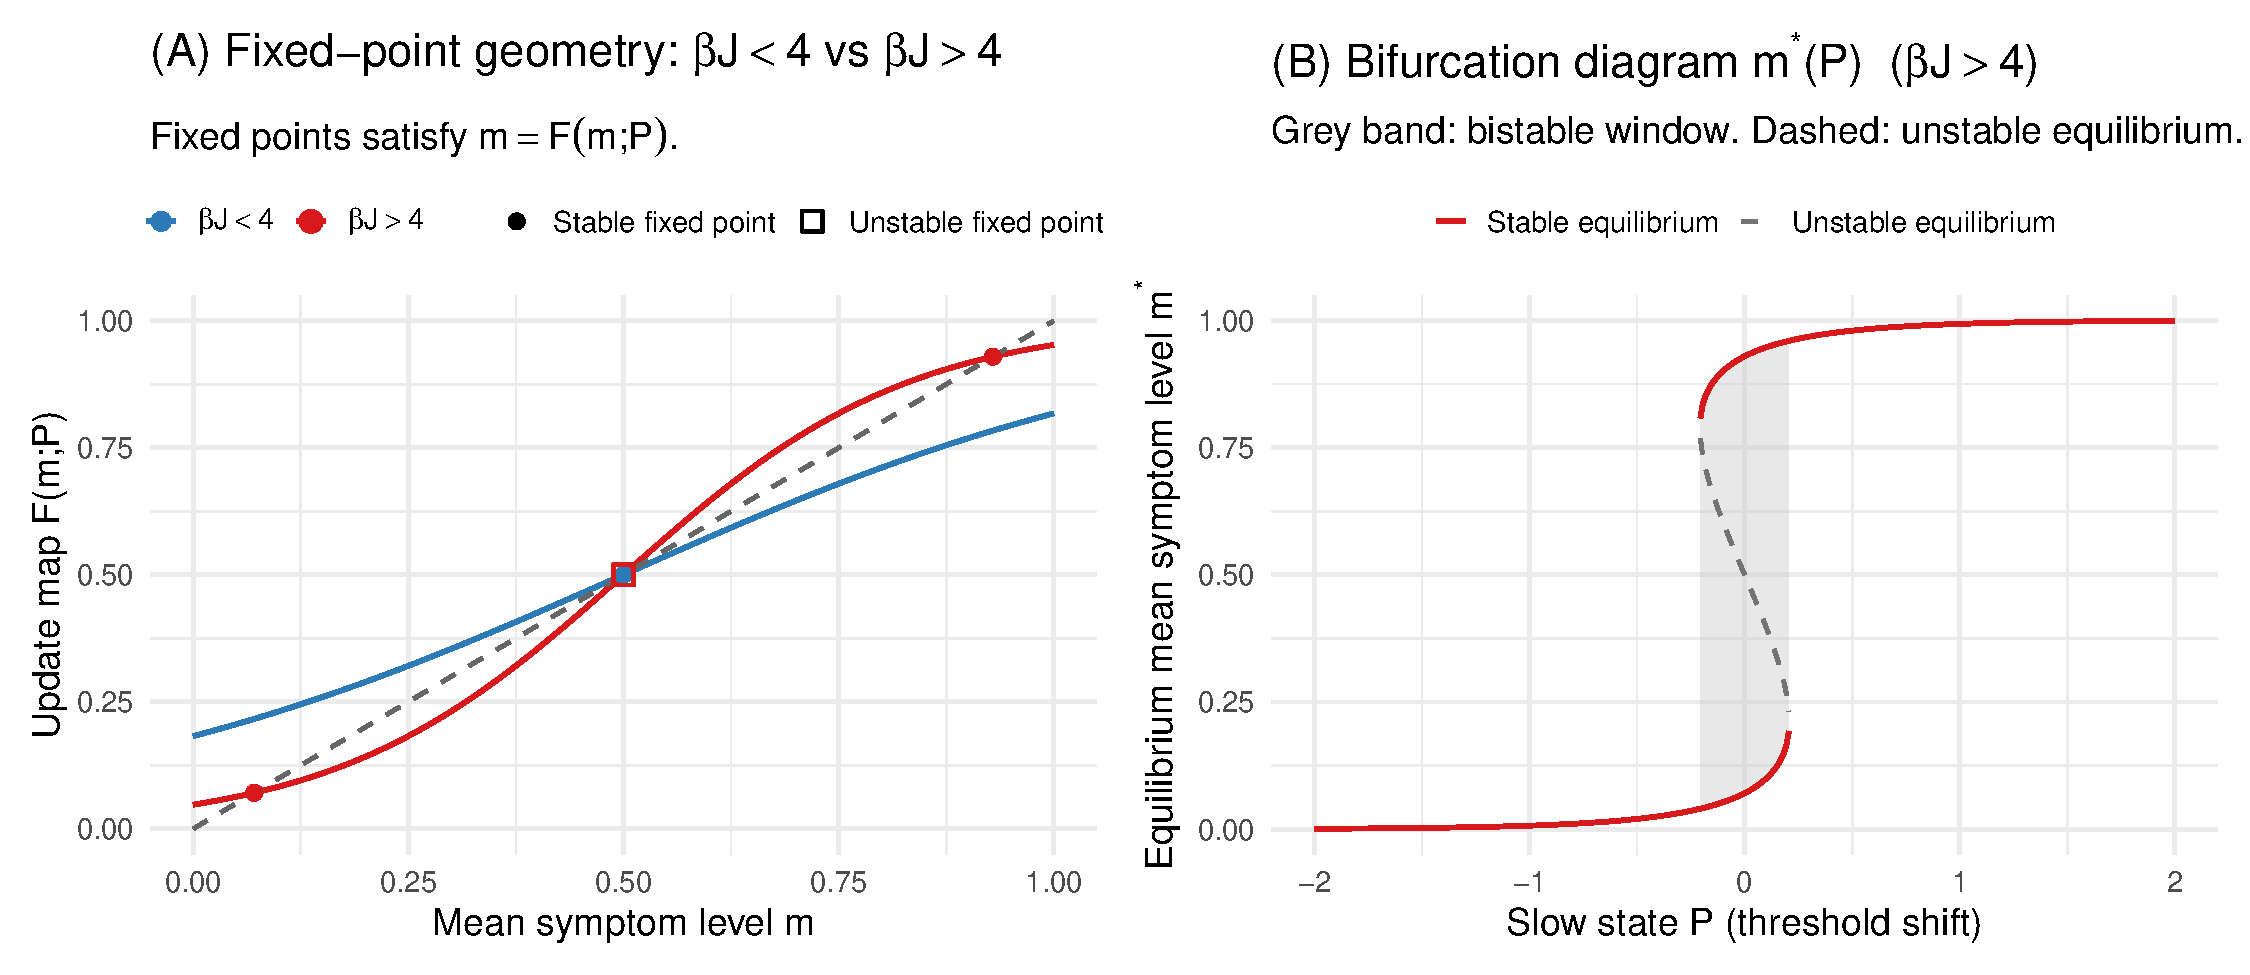
\includegraphics[width=\linewidth]{figs/Figure_AB_fixedpoints_bifurcation_v2.pdf}
  \caption{\textbf{Geometric intuition for bistability in the 0/1 Curie--Weiss fast layer.}
  \textbf{(A)} For a fixed slow state \(P\), the fast layer defines an update rule \(m \mapsto F(m;P)\). Fast-layer equilibria are fixed points where the update returns the same value, \(m^\ast = F(m^\ast;P)\), which appear as intersections of the curve \(y=F(m;P)\) with the diagonal \(y=m\). Whether an intersection is stable or unstable is determined by the local slope at the crossing: if the update curve is flatter than the diagonal, nearby values are pulled back toward \(m^\ast\) (stable); if it is steeper, nearby values are pushed away (unstable). When \(\beta J<4\), the curve is never steep enough to create more than one crossing, so there is a single stable fixed point. When \(\beta J>4\), the curve can become steep enough near the middle to produce three crossings for an appropriate range of \(P\), yielding two stable outer fixed points separated by one unstable middle fixed point. \textbf{(B)} Panel B keeps \(\beta J>4\) fixed and varies \(P\). Changing \(P\) shifts the update curve in Panel A, so the intersection points move with \(P\). Plotting the resulting fixed points \(m^\ast(P)\) produces the bifurcation diagram: solid curves track the stable fixed points and the dashed curve tracks the unstable middle fixed point. The grey band marks the range of \(P\) values where two stable equilibria coexist. At the band edges (folds), one stable branch disappears; under slow drift in \(P\), this forces rapid jumps between the low- and high-symptom branches and yields hysteresis.}
  \label{fig:fixedpoints_bifurcation}
\end{figure}
\subsection{Coupling across timescales}
The model therefore contains two coupled loops. The first is the slow-to-fast pathway: the slow state \(P_t\) shifts the ease with which symptoms become active. In a monostable fast layer, this produces gradual changes in symptom level. In a bistable-capable fast layer, the same slow shift can instead move the system toward a transition boundary, where a small additional change may trigger a large jump in symptoms.
The second loop is the fast-to-slow pathway: sustained symptom elevation feeds back into \(P_t\) through \(m_{\mathrm{slow},t}\). When \(b>0\), prolonged symptom activation pushes the slow state upward. This creates a reinforcement loop across timescales: symptoms worsen the slow state, and the worsened slow state makes symptoms easier to activate. Acute stressors act on this same slow state. Their effect is therefore regime-dependent. Far from a transition boundary, a stressor may produce only temporary worsening. Near a boundary, the same kind of perturbation may be enough to move the system into a persistent high-symptom state.
% ================================================
% Simulation design + results (final story: A, A+S, B, B+S)
% ================================================
\section{Simulation design}\label{sec:simulation}
The model suggests that threshold shifts can have different consequences depending on two features: the equilibrium structure of the fast layer and the way the slow state changes over time. The fast layer may have a single stable symptom level, in which case changes in the slow state should produce gradual changes in symptoms, or it may support both low- and high-symptom states, in which case the same slow shift can produce abrupt transitions. The slow state may also change only gradually, or it may be displaced by acute stressors.
We use these two features to construct four diagnostic scenarios. In each scenario, two groups differ in their baseline level of the slow state, while the fast-layer interaction parameters are held fixed across groups. The scenarios therefore ask what kinds of between-group differences can arise from slow-state dynamics alone, without changing symptom--symptom coupling. They are not intended to exhaust all clinically realistic possibilities; rather, they separate the roles of equilibrium structure and acute stressors under fixed coupling. Although they are not disorder-specific, each can be understood as representing a familiar clinical pattern.
\subsection{Scenario set}\label{sec:sim_scenarios}
\begin{itemize}[leftmargin=*]
\item \textbf{Monostable separation (M; \(\beta J<4\), no acute stressors):} the fast layer is monostable and the slow state evolves without discrete stressors. This is the simplest case: groups differ in their baseline level of the slow state, producing stable differences in symptom levels, but changes remain gradual. Clinically, one can think of two groups that differ in ongoing background adversity or precarity, leading one group to show consistently higher symptom levels than the other, but without abrupt episodes or switching.
\item \textbf{Monostable separation with acute stressors (M+S; \(\beta J<4\), acute stressors):} this scenario adds discrete stressors to the slow state while keeping the fast layer monostable. Symptom levels can increase abruptly following a stressor, but the increase is temporary rather than the start of a more persistent episode. Clinically, this resembles a person or group facing occasional acute stressors, such as a conflict, financial difficulty, or a brief health problem, which temporarily intensify symptoms but do not trigger a lasting episode.
\item \textbf{Bistable switching (B; \(\beta J>4\), no acute stressors):} here, the fast layer is bistable-capable, so gradual changes in the slow state can eventually produce abrupt shifts in symptom levels. The key point is that no single acute stressor is required; slow accumulation and symptom-to-slow-state feedback alone can move the system into a different regime and help maintain it. Clinically, this resembles a pattern in which pressures build up over time, for example, through prolonged financial insecurity, caregiving strain, social isolation, or ongoing work stress. Symptoms may remain relatively low for a long period, but as these pressures accumulate, the person reaches a point at which symptom levels shift abruptly and remain elevated.
\item \textbf{Bistable switching with acute stressors (B+S; \(\beta J>4\), acute stressors):} this scenario combines bistability with discrete stressors. Here, the system is already closer to a transition, so an acute stressor can push symptom levels across that boundary. Clinically, this resembles a person who is already under growing strain, for example, because of chronic relationship tension, job insecurity, or persistent exhaustion, and then experiences an acute stressor such as an argument, a setback at work, or bad medical news. The stressor can trigger the episode, and if symptoms remain elevated, the resulting difficulties in functioning, such as poorer performance at work or more tension in relationships, can further worsen the slow state. This feedback can then help maintain the episode.
\end{itemize}
\subsection{Simulation settings}\label{sec:sim_protocol}
In each scenario, we simulate two groups defined by different baseline levels of the slow state, \(P_{\text{base}}\), which we refer to as the low-baseline and high-baseline groups. Within each scenario family, fast-layer parameters are held fixed across these groups so that between-group differences arise from the slow-state process rather than from changes in symptom interaction strength. When shocks are enabled, they affect the model only through sudden jumps in the slow state \(P_t\).
Simulations run for \(T=8000\) slow steps, with a burn-in of 500 steps and \(n_{\mathrm{rep}}=50\) replicates per group. The initial conditions are \(P_0=0\) and \(m_0=0.05\). Table~\ref{tab:scenario_design} summarizes the parameter values used in the simulations. The monostable scenarios use \(\beta J<4\), whereas the bistable-switching scenarios use \(\beta J>4\). Detailed parameter settings are reported in Appendix~A.
\definecolor{bandgray}{gray}{0.97}
\definecolor{rulegray}{gray}{0.80}
\newcolumntype{L}[1]{>{\raggedright\arraybackslash}m{#1}}
\begin{table}[htbp]
\centering
\begin{threeparttable}
\caption{Simulation scenarios and shared settings.}
\label{tab:scenario_design}
\footnotesize
\setlength{\tabcolsep}{6pt}
\renewcommand{\arraystretch}{1.15}
\begin{tabularx}{\linewidth}{@{} L{2.4cm} L{3.1cm} X @{}}
\toprule
\rowcolor{bandgray}
\multicolumn{3}{c}{\textit{Shared across all scenarios}} \\
\arrayrulecolor{rulegray}\specialrule{0.4pt}{0pt}{0pt}
\textbf{Category} & \textbf{Setting} & \textbf{Value} \\
\arrayrulecolor{rulegray}\specialrule{0.4pt}{0pt}{0pt}
\textit{Groups}
  & Baseline slow-state levels
  & Low-baseline group: \(P_{\text{base}}=-0.506\); high-baseline group: \(P_{\text{base}}=0.106\). \\
\textit{Slow state}
  & Shared parameters
  & \(\kappa=0.20,\; b=0.15,\; \sigma_P=0.04,\; \lambda_m=0.001,\; m_\star=0.25,\; \gamma=1,\; h=0\). \\
\textit{Fast layer}
  & Shared size and updating
  & \(N=100\); \(40\) sweeps per step. \\
\textit{Simulation}
  & Time grid and run length
  & \(dt=0.02\); \(T=8000\) slow steps; burn-in \(=500\); \(n_{\mathrm{rep}}=50\) replicates per group. \\
\textit{Initialization}
  & Initial conditions
  & \((P_0,m_0)=(0,0.05)\). \\
\midrule
\rowcolor{bandgray}
\multicolumn{3}{c}{\textit{Scenario-specific settings}} \\
\arrayrulecolor{rulegray}\specialrule{0.4pt}{0pt}{0pt}
\textbf{Scenario} & \textbf{Acute stressors} & \textbf{Fast layer} \\
\arrayrulecolor{rulegray}\specialrule{0.4pt}{0pt}{0pt}
\textit{M}
  & Off
  & Monostable (\(\beta=1.0,\; J=2.5,\; \beta J=2.5<4\)) \\
\textit{M+S}
  & On
  & Monostable (\(\beta=1.0,\; J=2.5,\; \beta J=2.5<4\)) \\
\textit{B}
  & Off
  & Bistable-capable (\(\beta=2.0,\; J=3.0,\; \beta J=6.0>4\)) \\
\textit{B+S}
  & On
  & Bistable-capable (\(\beta=2.0,\; J=3.0,\; \beta J=6.0>4\)) \\
\arrayrulecolor{black}\bottomrule
\end{tabularx}
\vspace{2mm}
\begin{tablenotes}[flushleft]
\footnotesize
\item \textit{Note.} Each scenario--group--replicate combination was assigned a deterministic seed using \texttt{L'Ecuyer-CMRG}. Detailed acute-stressor parameter settings and implementation are described in Appendix~A.
\end{tablenotes}
\end{threeparttable}
\end{table}
We summarize the simulations in four complementary ways. First, we show representative trajectories over time. Second, we project simulated trajectories onto the fast-layer equilibrium structure \(m^*(P)\). Third, we summarize behavior across replicates in terms of symptom level, slow state, time spent in the high-symptom state, and switching between low- and high-symptom states. Fourth, we compute heatmaps over \((\beta J, P_{\text{base}})\) under a standardized no-stressor protocol to show the broader regime structure of the model.
To summarize time spent in low- and high-symptom states and the number of transitions between them, we convert the continuous symptom-level signal \(m_t\) into a binary state sequence \(z_t\in\{0,1\}\) using a two-threshold rule with memory.\footnote{We use \(m_{\mathrm{low}}=0.30\) and \(m_{\mathrm{high}}=0.70\) to define low and high states for summary purposes only. These cutoffs are not part of the model dynamics; they are used only to summarize simulated trajectories in terms of sustained low- and high-symptom episodes. Using two separate thresholds avoids counting brief fluctuations around the middle of the range as repeated switches.} The purpose of this rule is to capture clear moves between low- and high-symptom states rather than counting every small fluctuation in \(m_t\). Values below the lower threshold are labeled low, values above the upper threshold are labeled high, and values in between inherit the previous label:
\[
z_t=
\begin{cases}
0, & m_t \le m_{\mathrm{low}},\\[4pt]
1, & m_t \ge m_{\mathrm{high}},\\[4pt]
z_{t-1}, & m_{\mathrm{low}} < m_t < m_{\mathrm{high}},
\end{cases}
\qquad
m_{\mathrm{low}}=0.30,\quad m_{\mathrm{high}}=0.70.
\]
\noindent Let \(T_{\mathrm{post}}\) denote the number of post-burn-in time points. We define high-state occupancy as
\[
f_{\mathrm{high}}
=
\frac{1}{T_{\mathrm{post}}}\sum_{t=1}^{T_{\mathrm{post}}} z_t,
\]
that is, the fraction of post-burn-in time the trajectory spends in the high state.
\noindent We define the switching count as the number of times the labeled state changes:
\[
N_{\mathrm{switch}}
=
\sum_{t=2}^{T_{\mathrm{post}}} \mathbf{1}\!\left(z_t \neq z_{t-1}\right),
\]
where \(\mathbf{1}(\cdot)\) is the indicator function. For the heatmaps, \(f_{\mathrm{high}}\) and \(N_{\mathrm{switch}}\) are computed for each replicate and then averaged across replicates at each \((\beta J, P_{\text{base}})\) grid point.
\subsection{Network-estimation check}\label{sec:network_estimation_check}
The diagnostic simulations above show how slow context can produce different symptom trajectories under fixed reinforcement. We next add a compact estimation check that asks a more direct network-comparison question: if two groups are generated with the same symptom--symptom coupling but different slow-context regimes, do their estimated symptom networks appear different?
Because the mean-field model summarizes symptom reinforcement with a single parameter \(J\), it is useful for analyzing equilibrium structure but not for asking how individual symptom edges are recovered. For this estimation check only, we therefore use a pairwise extension of the fast layer. This extension is not intended to replace the mean-field model. It is used only to ask whether a standard symptom-network estimator attributes shared slow-context variation to symptom--symptom edges when slow context is omitted from the analysis.
In the pairwise data-generating model, symptom \(i\)'s activation tendency is
\[
\operatorname{logit}\Pr(S_i=1\mid \mathbf S_{-i},P)
=
h_i+\sum_{j\neq i}W^{\mathrm{true}}_{ij}S_j+\gamma_iP .
\]
The matrix \(W^{\mathrm{true}}\) is held fixed across groups. The groups differ only in the distribution of the slow context \(P\). We then estimate symptom networks in two ways. First, we estimate the network from symptoms alone,
\[
\operatorname{logit}\Pr(S_i=1\mid \mathbf S_{-i})
=
\alpha_i+\sum_{j\neq i}\widehat W^{\mathrm{omit}}_{ij}S_j .
\]
Second, we estimate the network while including the slow context as an additional predictor,
\[
\operatorname{logit}\Pr(S_i=1\mid \mathbf S_{-i},P)
=
\alpha_i+\widehat\gamma_iP+\sum_{j\neq i}\widehat W^{\mathrm{adj}}_{ij}S_j .
\]
We compare the two estimators in terms of estimated global strength,
\(\mathrm{GS}=\sum_{i<j}|\widehat W_{ij}|\), and recovery error relative to the known coupling
matrix \(W^{\mathrm{true}}\), defined as the mean absolute deviation between estimated and true
edges,
\[
\mathrm{MAE}=\binom{N}{2}^{-1}\sum_{i<j}\bigl|\widehat W_{ij}-W^{\mathrm{true}}_{ij}\bigr| .
\]
Because \(W^{\mathrm{true}}\) is fixed and known, any increase in estimated connectivity or
recovery error under the symptom-only estimator reflects distortion introduced by omitting the
slow context rather than a change in the data-generating symptom--symptom coupling.
To connect this check to the slow--fast argument, and to test it directly against the paper's own
coupled dynamics rather than an exogenous stand-in, we generated the slow context \(P\) not as an
independently sampled covariate but from the model's own feedback equation
(Eq.~\eqref{eq:slow_update}): each simulated individual ran their own private coupled fast/slow
system, exactly as in the main scenario simulations. We varied two things that jointly determine
how much of this coupled process an observer actually sees: the model's own diffusion parameter
\(\sigma_P\), which sets how much individuals' context naturally varies, and the length of the
observation window \(W\) used to construct each measurement, from a single near-instantaneous
snapshot to long temporal aggregation. The identification problem should be weakest when
\(\sigma_P\) is small or \(W\) is long (observations contain little slow-context variation), and
strongest when \(\sigma_P\) is large and \(W\) is short (observations preserve the full
between-person spread of an unmodeled contextual process). Full implementation details, including
the exact \(\sigma_P\) and \(W\) grids, the window-averaging definition, and the network-generation
parameters, are reported in Appendix~\ref{app:network_check_details}.
% ===========================================================
% Results
% ===========================================================
\section{Results}\label{sec:results}
The simulations show how the same fast symptom system can produce different kinds of between-group differences depending on the slow-state regime in which it is embedded. We present the results in four steps. First, we show what happens when the fast layer has only one stable symptom level. Second, we add acute stressors to this monostable setting. Third, we allow the fast layer to support both low- and high-symptom states. Finally, we add acute stressors to this bistable-capable setting. This sequence separates two questions: whether the fast layer changes smoothly or can tip between regimes, and whether changes in the slow state arise gradually or can also occur through sudden stressors. In all figures, green denotes the low-baseline group and red denotes the high-baseline group.
% \section{Results}\label{sec:results}
% We present the results by scenario so that the effects of the two main design features can be seen step by step: first whether the fast layer is monostable or bistable-capable, and second whether acute stressors are absent or present. This makes it easier to see what changes when acute stressors are added, and what changes when the fast layer can support two stable states. In all figures, green denotes the low-baseline group and red denotes the high-baseline group.
% --------------------------------
% Fig 1: 2x2 representative time series (M, M+S, B, B+S)
% --------------------------------
\begin{figure}[htbp]
  \centering
\makebox[\textwidth][c]{%
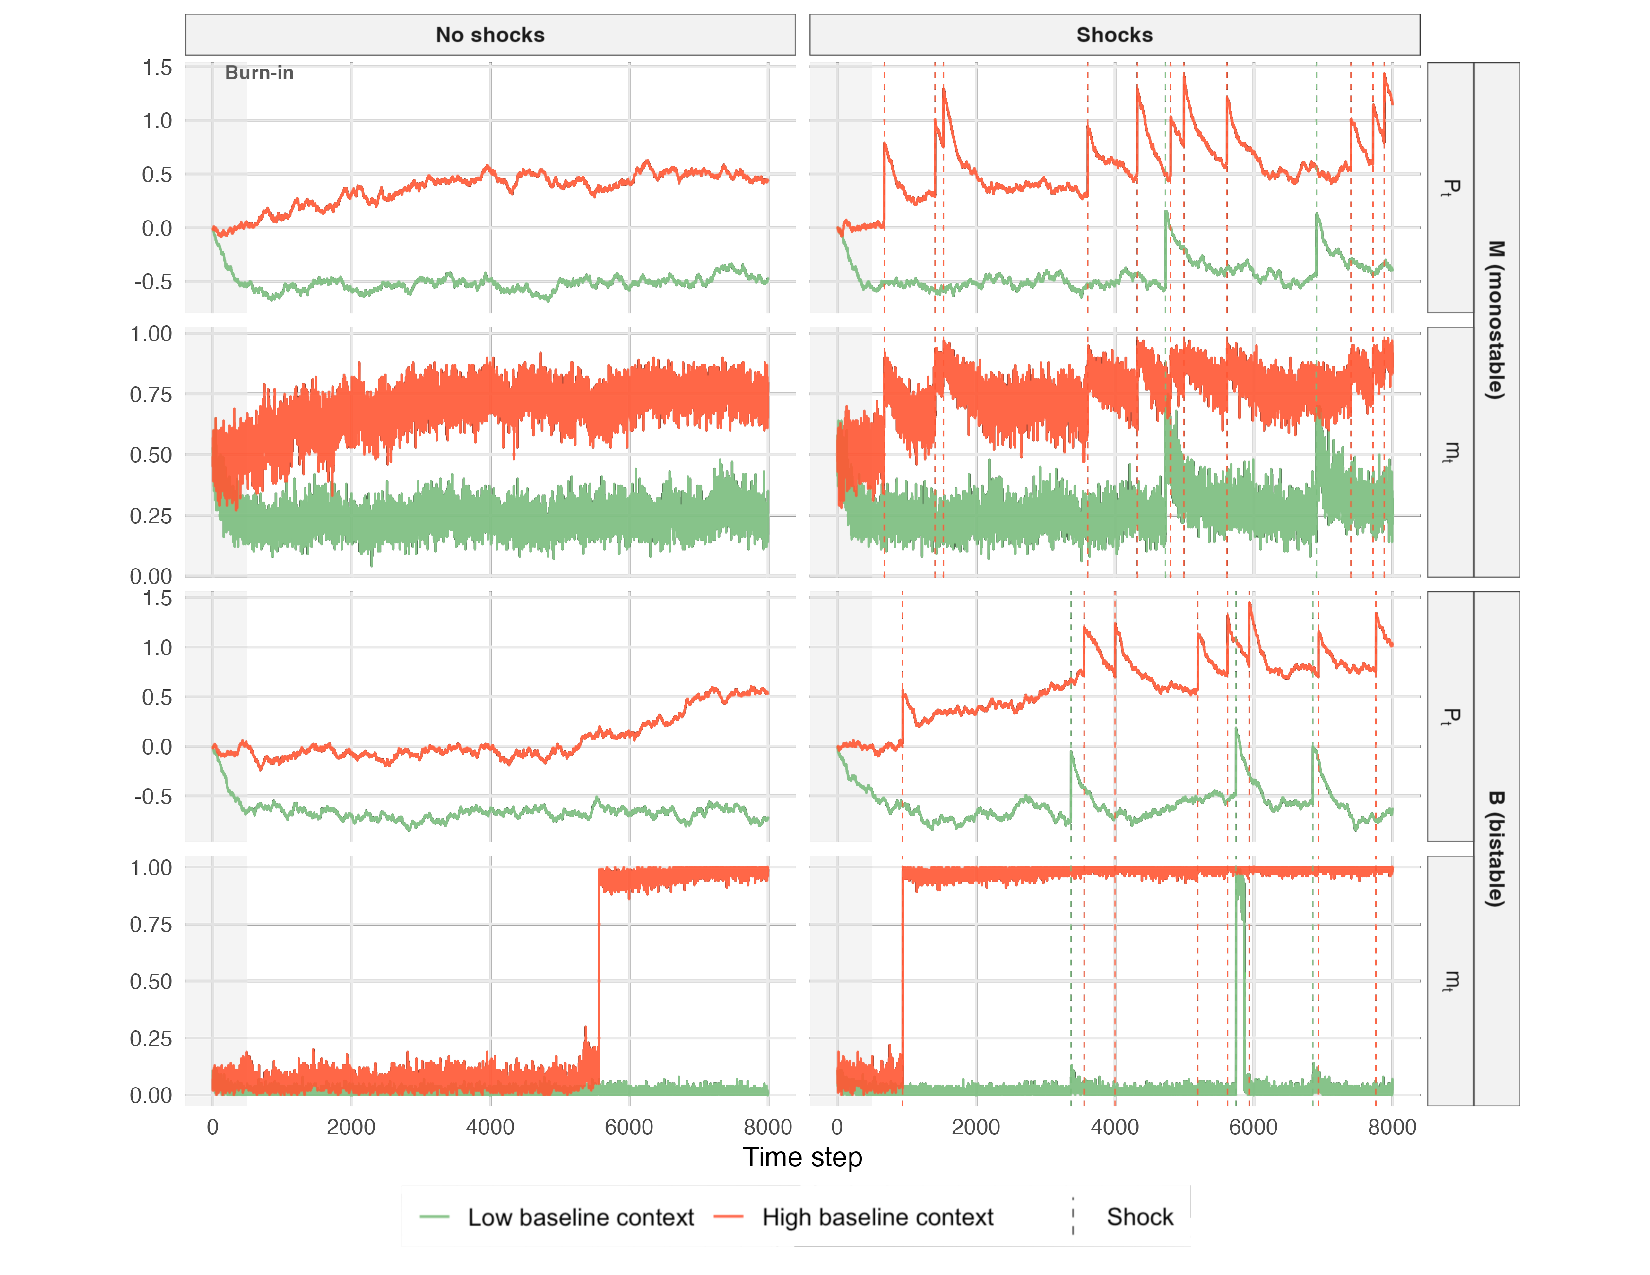
\includegraphics[width=1\textwidth]{figs/Figure_timeseries_4panel_M.pdf}}
\caption{\textbf{Representative trajectories of \(P_t\) and \(m_t\) across the four focal scenarios.}
Columns compare no-acute-stressor and acute-stressor conditions, and rows compare the monostable and bistable-capable regimes. In each panel, the upper trace shows the slow state \(P_t\) and the lower trace shows the mean symptom level \(m_t\); green and red correspond to the low- and high-baseline groups, respectively. Vertical dashed lines mark acute stressor times in the acute-stressor scenarios.
In the monostable regime (top row), baseline differences in the slow state produce stable separation in symptom levels. With no acute stressors (top-left), both groups fluctuate around distinct levels without regime change. When acute stressors are added (top-right), they produce abrupt perturbations in \(P_t\) and corresponding short-lived responses in \(m_t\), but trajectories return toward their group-specific range because the fast layer remains monostable.
In the bistable-capable regime (bottom row), the dynamics change qualitatively. Without acute stressors (bottom-left), the high-baseline group enters the high-symptom state late in the run, while the low-baseline group remains in the low-symptom state. This transition is accompanied by gradual upward drift in \(P_t\), reflecting slow feedback from sustained symptom elevation onto the slow state. When acute stressors are added (bottom-right), transitions into the high-symptom state occur earlier and more readily. Even the low-baseline group shows brief symptom increases following acute stressors, whereas the high-baseline group is more readily pushed into the high-symptom state and remains there for longer periods.}
  \label{fig:sim_timeseries}
\end{figure}
\subsection{Monostable separation without acute stressors (M)}\label{sec:res_M}
The simplest case shows that threshold shifts alone can produce stable group separation. The two groups have the same fast-layer parameters, but their slow states return toward different baseline values. Because the slow state shifts the overall ease of symptom activation, the groups settle around different symptom levels (Fig.~\ref{fig:sim_timeseries}, top-left). In the monostable regime, this separation remains smooth: each value of the slow state corresponds to a single expected symptom level, and the simulated trajectories follow that single equilibrium relation (Fig.~\ref{fig:sim_overlay}, top-left). Across replicates, the two groups remain separated but do not show sustained switching into a different symptom regime (Fig.~\ref{fig:sim_ensemble}, top-left).
\subsection{Monostable separation with acute stressors (M+S)}\label{sec:res_MS}
Adding acute stressors changes the short-term variability but not the qualitative regime. Stressors produce sudden increases in the slow state and corresponding temporary increases in symptom level (Fig.~\ref{fig:sim_timeseries}, top-right). However, because the fast layer still has only one stable symptom level for each slow-state value, these perturbations do not produce lasting transitions. The trajectories are displaced along the same equilibrium relation and then return toward their group-specific range (Fig.~\ref{fig:sim_overlay}, top-right). Across replicates, this appears as broader fluctuation, especially in the high-baseline group, but not as prolonged high-symptom episodes or systematic switching (Fig.~\ref{fig:sim_ensemble}, top-right).
\subsection{Bistable switching without acute stressors (B)}\label{sec:res_B}
The dynamics change once the fast layer can support both low- and high-symptom states. In this setting, no acute stressor is needed for a transition to occur. Continuous slow-state fluctuations, together with symptom-to-slow-state feedback, can gradually move the system toward a transition boundary. This occurs most clearly in the high-baseline group, which eventually shifts from the low-symptom state to the high-symptom state (Fig.~\ref{fig:sim_timeseries}, bottom-left). In the equilibrium projection, this transition corresponds to movement through the bistable window and onto the high-symptom branch (Fig.~\ref{fig:sim_overlay}, bottom-left). Across replicates, the mean symptom level rises gradually because an increasing fraction of high-baseline trajectories enter the high-symptom state over time (Fig.~\ref{fig:sim_ensemble}, bottom-left).
\subsection{Bistable switching with acute stressors (B+S)}\label{sec:res_BS}
When acute stressors are added to the bistable-capable setting, transitions occur earlier and more often. The key difference from the monostable stressor scenario is that the system can now be pushed across a transition boundary. Because the high-baseline group is already closer to that boundary, stressor-driven increases in the slow state more readily move the symptom layer onto the high-symptom branch (Fig.~\ref{fig:sim_timeseries}, bottom-right). In the equilibrium projection, these events appear as larger shifts in \(P_t\) that cross the fold region (Fig.~\ref{fig:sim_overlay}, bottom-right). At the ensemble level, the high-baseline group shows an earlier and steeper rise in mean symptom level, indicating that more replicates enter the high-symptom state and do so sooner (Fig.~\ref{fig:sim_ensemble}, bottom-right).
% --------------------------------
% Fig 2: 2x2 equilibrium overlay (M, M+S, B, B+S)
% --------------------------------
\begin{figure}[htbp]
  \centering
  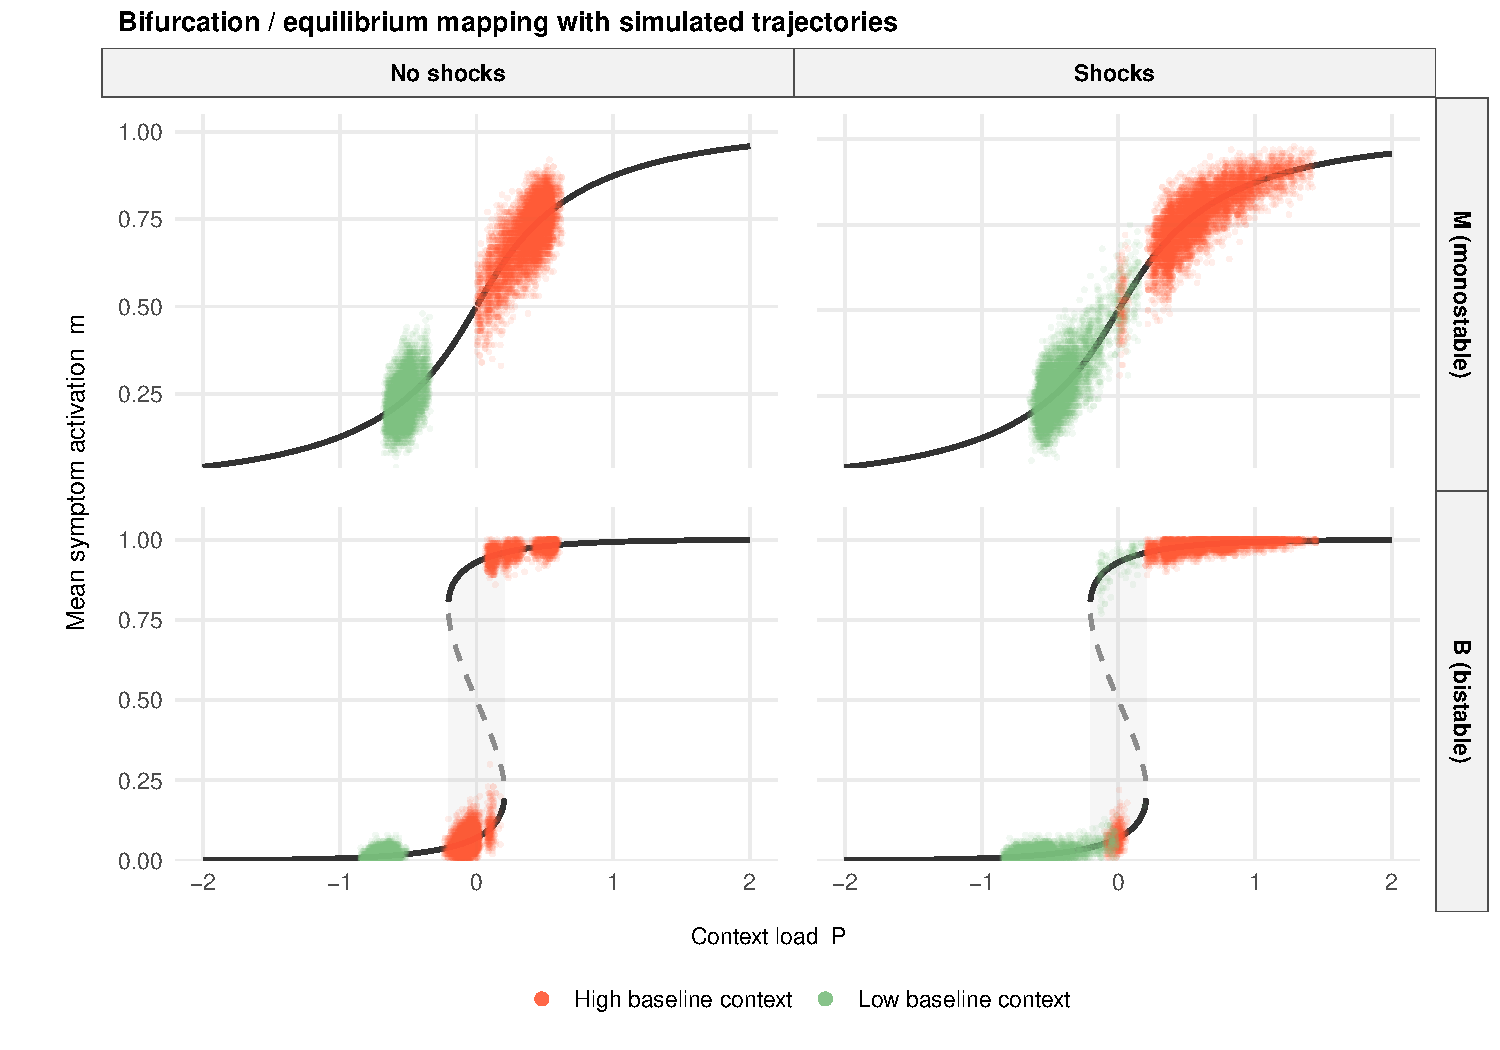
\includegraphics[width=1\textwidth]{figs/Figure_overlay_4panel_M.pdf}
\caption{\textbf{Simulated trajectories projected onto the fast-layer equilibrium structure \(m^\ast(P)\).}
Each point shows the simulated symptom level \(m_t\) plotted against the corresponding slow-state value \(P_t\). The black curve indicates the mean-field equilibrium relation \(m^\ast(P)\) for the fast layer; dashed segments mark unstable branches in the bistable-capable regime. Colors indicate the low- and high-baseline groups.
In the monostable regime (top row), trajectories follow a single-valued relation between slow state and symptom level. Without acute stressors (top-left), the two groups occupy different parts of the same equilibrium curve because their baseline slow states differ. With acute stressors (top-right), trajectories are temporarily displaced along this curve but remain on the same branch.
In the bistable-capable regime (bottom row), the equilibrium structure contains two stable branches separated by an unstable middle segment. Without acute stressors (bottom-left), trajectories for the high-baseline group eventually move from the low-symptom branch to the high-symptom branch as the slow state evolves. With acute stressors (bottom-right), larger stressor-driven changes in \(P_t\) more readily push trajectories across the fold region, leading to earlier and more frequent moves onto the high-symptom branch.}
  \label{fig:sim_overlay}
\end{figure}
% --------------------------------
% Fig 3: ensemble ribbons (m and P) by scenario
% --------------------------------
\begin{figure}[htbp]
  \centering
  \includegraphics[width=0.9\textwidth]{figs/Figure_ensemble_ribbons_M.pdf}
\caption{\textbf{Across-replicate summaries of \(P_t\) and \(m_t\) by scenario and group.}
Columns compare no-acute-stressor and acute-stressor conditions, and rows compare the monostable and bistable-capable regimes. In each panel, faint lines show individual replicates, solid lines show the across-replicate mean, and shaded ribbons indicate the central quantile range. Green and red correspond to the low- and high-baseline groups, respectively.
In the monostable regime (top row), the two groups remain stably separated in both slow state and symptom level. Without acute stressors (top-left), the means stay well separated and variability remains modest. With acute stressors (top-right), the mean trajectories remain similar but variability increases, especially for the high-baseline group, reflecting short-lived stressor responses without persistent regime change.
In the bistable-capable regime (bottom row), the ensemble patterns change qualitatively. Without acute stressors (bottom-left), the mean symptom level for the high-baseline group rises gradually over time, indicating that an increasing fraction of replicates enter the high-symptom state as the slow state evolves, while the low-baseline group remains near the low-symptom state. With acute stressors (bottom-right), this shift occurs earlier and more strongly: the high-baseline group moves rapidly toward near-complete occupancy of the high-symptom state, while the low-baseline group remains mostly low but shows greater variability and occasional upward responses.}
  \label{fig:sim_ensemble}
\end{figure}
% --------------------------------
% Fig 4: heatmaps
% --------------------------------
\begin{figure}[htbp]
  \centering
  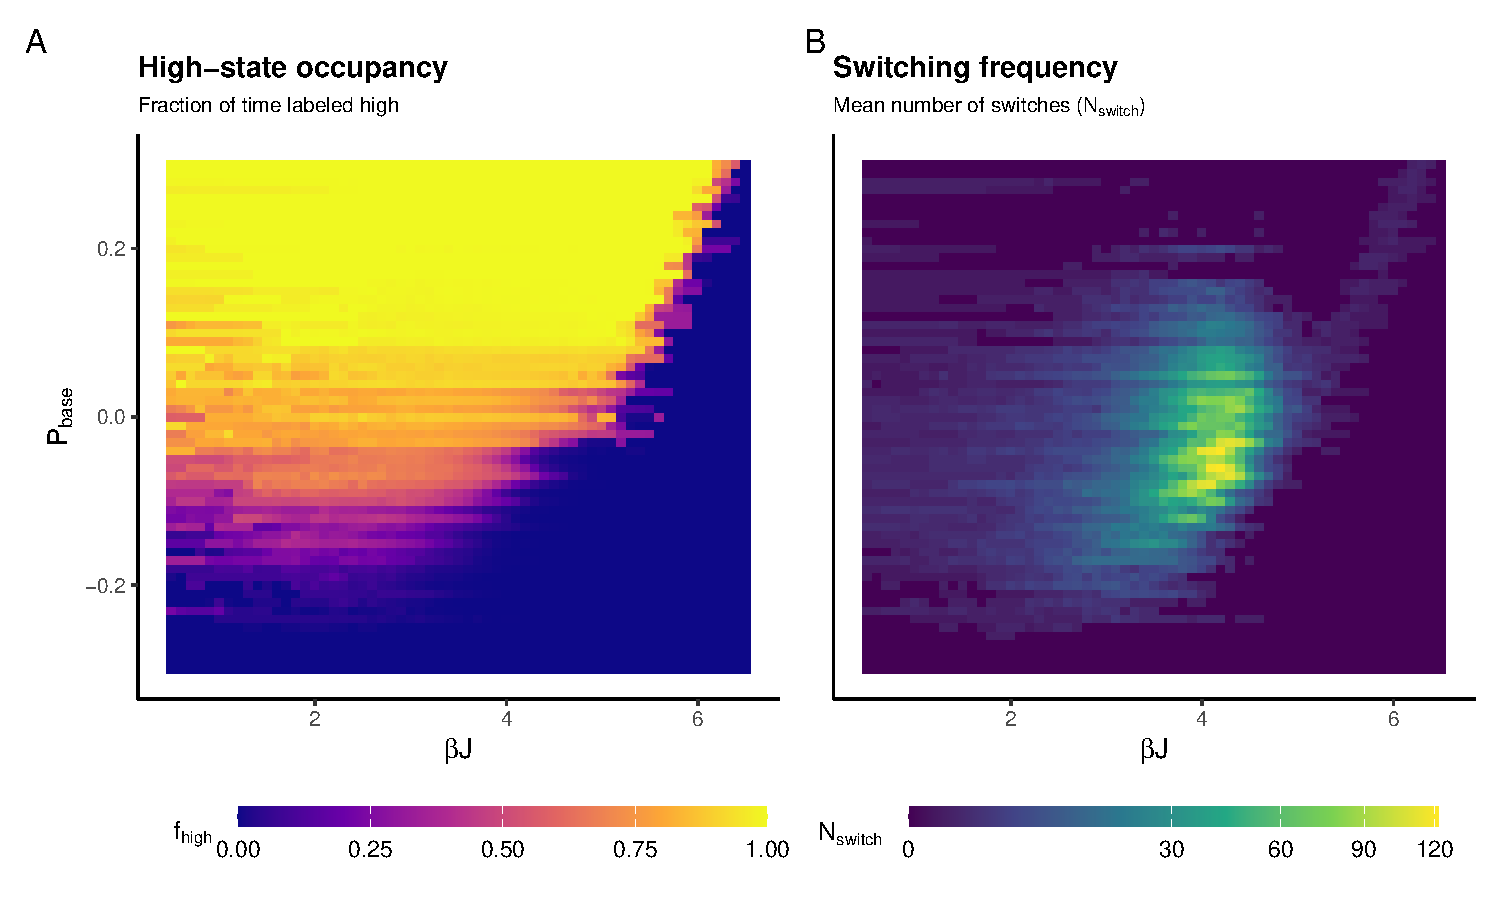
\includegraphics[width=\linewidth]{figs/Figure_heatmaps_2panel_plasma_clean.pdf}
\caption{\textbf{Regime maps (no acute stressors) over \((\beta J, P_{\text{base}})\).}
Heatmaps summarize replicate simulations across a grid of fast-layer reinforcement \(\beta J\) and baseline slow-state level \(P_{\text{base}}\), using the two-threshold state-labeling rule defined in the Simulation design section. \textbf{(A)} High-state occupancy, \(f_{\mathrm{high}}\), defined as the fraction of post-burn-in time labeled as high. High occupancy is concentrated in an intermediate region of parameter space rather than increasing monotonically across the grid. For low \(\beta J\) and low \(P_{\text{base}}\), trajectories remain mostly in the low-symptom state. As \(P_{\text{base}}\) increases, trajectories more often enter the high-symptom state, but at very large \(\beta J\) the map bends back toward lower occupancy because stronger self-reinforcement stabilizes the low-symptom branch over a broader range of \(P\). \textbf{(B)} Switching frequency, shown as the mean number of low\(\leftrightarrow\)high transitions \(N_{\mathrm{switch}}\) across replicates. Switching is rare in regions where trajectories remain mostly low or mostly high, and is concentrated in the intermediate band where occupancy is mixed.}
\label{fig:sim_heatmaps}
\end{figure}
\subsection{Regime maps over \((\beta J, P_{\text{base}})\)}\label{sec:res_heatmaps}
Figure~\ref{fig:sim_heatmaps} extends the no-acute-stressor scenarios to a broader parameter map. The heatmaps summarize no-acute-stressor simulations across a grid of the combined fast-layer self-reinforcement parameter \(\beta J\) and baseline slow-state level \(P_{\text{base}}\).
Panel~A shows high-state occupancy, \(f_{\mathrm{high}}\), that is, the fraction of post-burn-in time labeled as high under the two-threshold state-labeling rule. High-state occupancy is greatest in an intermediate region of the parameter space rather than increasing monotonically across the grid. For low \(\beta J\) and low \(P_{\text{base}}\), trajectories remain mostly in the low-symptom state. As \(P_{\text{base}}\) increases, trajectories more often enter the high-symptom state. At very large \(\beta J\), however, this pattern bends back toward lower occupancy. The reason is that stronger self-reinforcement stabilizes not only the high-symptom branch but also the low-symptom branch. As a result, trajectories that begin on the low branch can remain there over a broader range of baseline contexts, unless the slow state is pushed far enough to cross the upper fold and move onto the high-symptom branch.
Panel~B shows the mean number of low\(\leftrightarrow\)high transitions, \(N_{\mathrm{switch}}\), under the same labeling rule. Switching is rare in regions where trajectories remain mostly low or mostly high and is concentrated in the intermediate band where occupancy is mixed. For \(\beta J<4\), these transitions mainly reflect threshold crossings in noisy monostable trajectories. For larger \(\beta J\), they increasingly reflect movement between distinct low- and high-symptom branches.
Taken together, these results show that threshold shifts do not have a single fixed consequence. When the fast layer is monostable, differences in the slow state mainly produce stable separation between groups, and acute stressors produce temporary worsening. When the fast layer is bistable-capable, similar slow-state differences can place one group closer to a transition boundary, so that gradual drift or acute stressors more readily lead to abrupt and persistent shifts into a high-symptom state. The four scenarios therefore describe qualitatively different developmental patterns that can arise even when the fast-layer interaction structure is unchanged.
\subsection{Network-estimation check}\label{sec:res_network_check}
Figure~\ref{fig:network_check} summarizes the network-estimation check. All context variation
shown was generated by the model's own coupled feedback dynamics (Eq.~\eqref{eq:slow_update}),
not by an exogenous covariate, and jointly varies the model's diffusion parameter \(\sigma_P\) and
the observation-window length \(W\) (Section~\ref{sec:network_estimation_check}).
At the model's own calibrated diffusion (\(\sigma_P=0.04\)), the omitted-context bias was small
throughout, as expected given how little between-person context spread this value naturally
produces: at the shortest window the symptom-only estimator exceeded the context-adjusted
estimator by 0.08 (\(SE=0.03\)) in global strength, and by the longest window this gap was no
longer distinguishable from zero (\(-0.01\), \(SE=0.02\)).
As \(\sigma_P\) increased -- widening the range of context an individual's own coupled dynamics
naturally explores -- the same pattern held at every level, but with a far larger and more
reliable gap. At \(\sigma_P=0.65\), the shortest window showed a gap of 12.3 (\(SE=0.24\)) in
global strength, comparable in size to the effect an earlier, exogenously-generated version of
this check produced by directly fixing \(SD_P=1.0\); the gap shrank steadily and significantly
across every intermediate window length, to 10.8 (\(SE=0.20\)) at \(W/\tau_P=1\), 7.7
(\(SE=0.19\)) at \(W/\tau_P=5\), and 3.9 (\(SE=0.22\)) at \(W/\tau_P=20\). The intermediate levels
(\(\sigma_P=0.15,0.35\)) showed the identical qualitative pattern at proportionally intermediate
magnitudes (Fig.~\ref{fig:network_check}B).
Recovery error relative to \(W^{\mathrm{true}}\) followed the same pattern: at \(\sigma_P=0.65\)
the symptom-only estimator's excess error over the context-adjusted estimator fell from 0.132
(\(SE=0.002\)) at the shortest window to 0.024 (\(SE=0.002\)) at the longest, while at the
calibrated \(\sigma_P=0.04\) this gap was negligible throughout (Fig.~\ref{fig:network_check}C).
Example estimated networks at the largest \(\sigma_P\) and shortest window examined illustrate the
same pattern visually: the symptom-only network becomes much denser than the true coupling
structure, whereas the context-adjusted network remains visibly closer to it
(Fig.~\ref{fig:network_check_graphs}).
Together, these results show that a shared, unmodeled slow context -- generated entirely by the
model's own coupled dynamics, not an external stand-in -- can be absorbed into estimated symptom
networks as inflated overall connectivity and poorer recovery of the true coupling structure, and
that this distortion is a joint function of how much the context varies and how long observations
are aggregated over: it is strongest for a cross-sectional snapshot of a highly variable context
and weakest, or absent, once observations average over a window long relative to the context's own
timescale, consistent with treating the symptom-only estimator as marginalizing over an omitted
common cause \parencite{kruis2016three,marsman2018introduction}. This is the dynamic
generalization of that equivalence result: for a cross-sectional snapshot, the entire
between-observation variance in the slow context is available to be misattributed to
symptom--symptom coupling; under long temporal aggregation, that variance is averaged away and the
true coupling is recovered.
\begin{figure}[htbp]
  \centering
  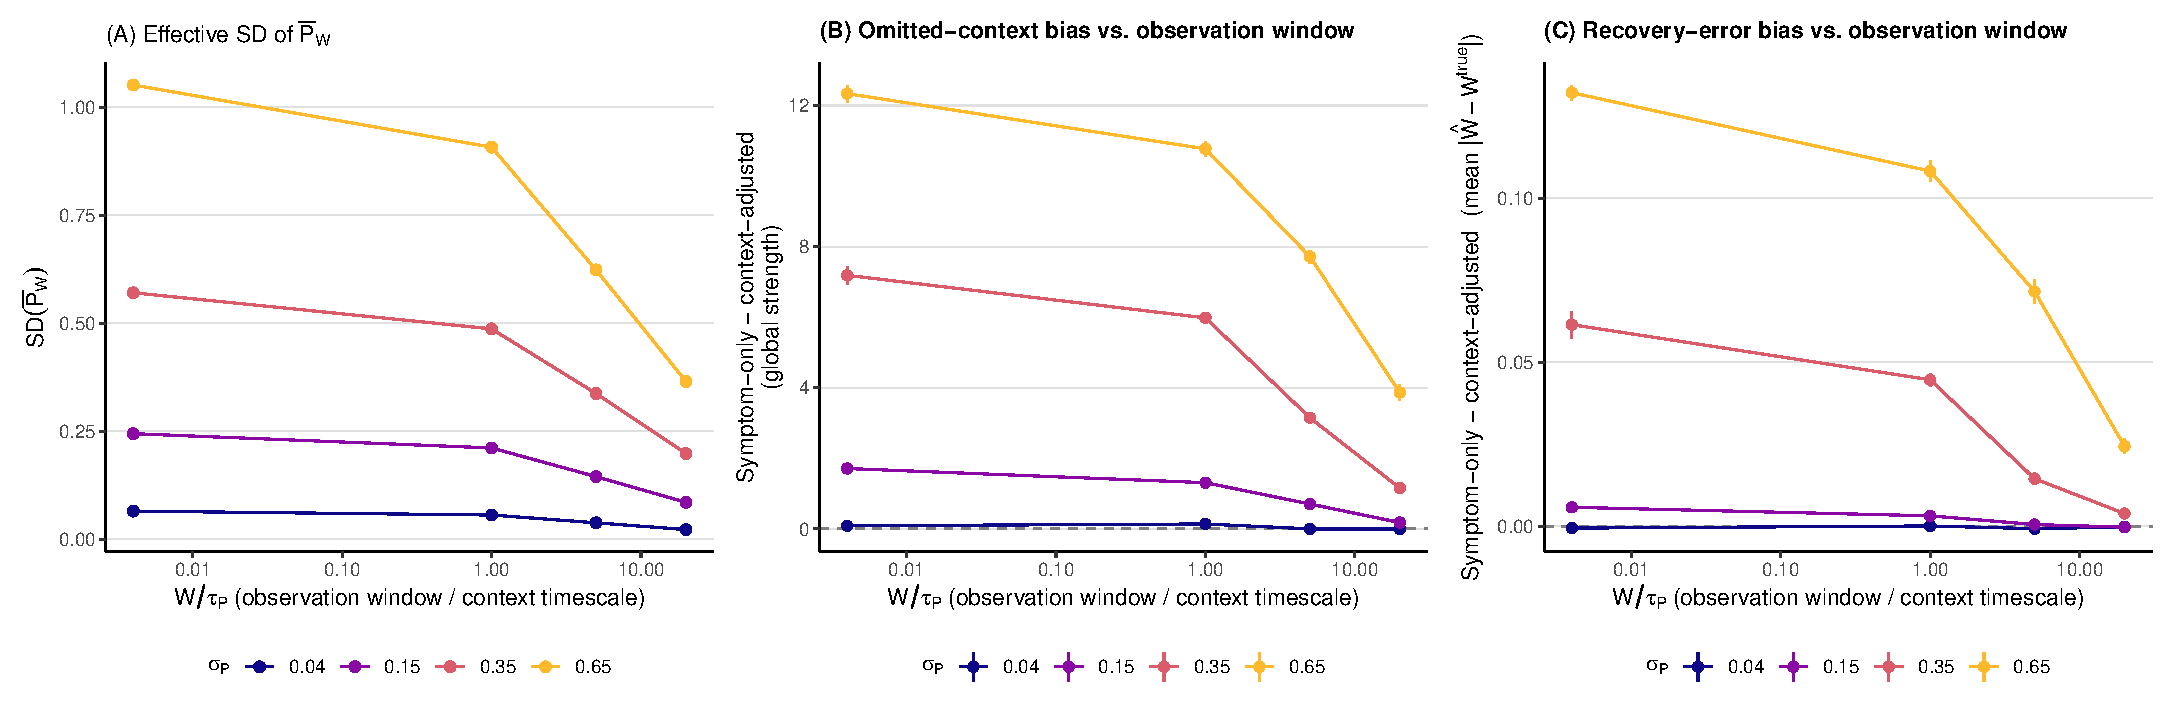
\includegraphics[width=\linewidth]{figs/Figure7_network_estimation_check.pdf}
  \caption{\textbf{Network-estimation check under the model's own coupled feedback dynamics.}
  Each simulated individual's slow context evolved under the real, coupled fast/slow model
  (Eq.~\eqref{eq:slow_update}), with feedback (\(b=0.15\)) active throughout; no exogenous context
  was used. Two things were varied: the model's own diffusion parameter \(\sigma_P\) (color, four
  levels from the calibrated value 0.04 up to 0.65), and the observation window \(W\) used to
  construct each measurement (x-axis, log scale, expressed as \(W/\tau_P\)).
  \textbf{(A)} Between-person standard deviation of the window-averaged context,
  \(SD(\bar P_W)\). \textbf{(B)} Omitted-context bias in estimated global strength (symptom-only
  minus context-adjusted, paired within data-generating network and replicate; error bars show
  \(\pm 1\ SE\)); the dashed line marks zero bias. \textbf{(C)} The same comparison for mean
  absolute recovery error relative to \(W^{\mathrm{true}}\).}
  \label{fig:network_check}
\end{figure}
\begin{figure}[htbp]
  \centering
  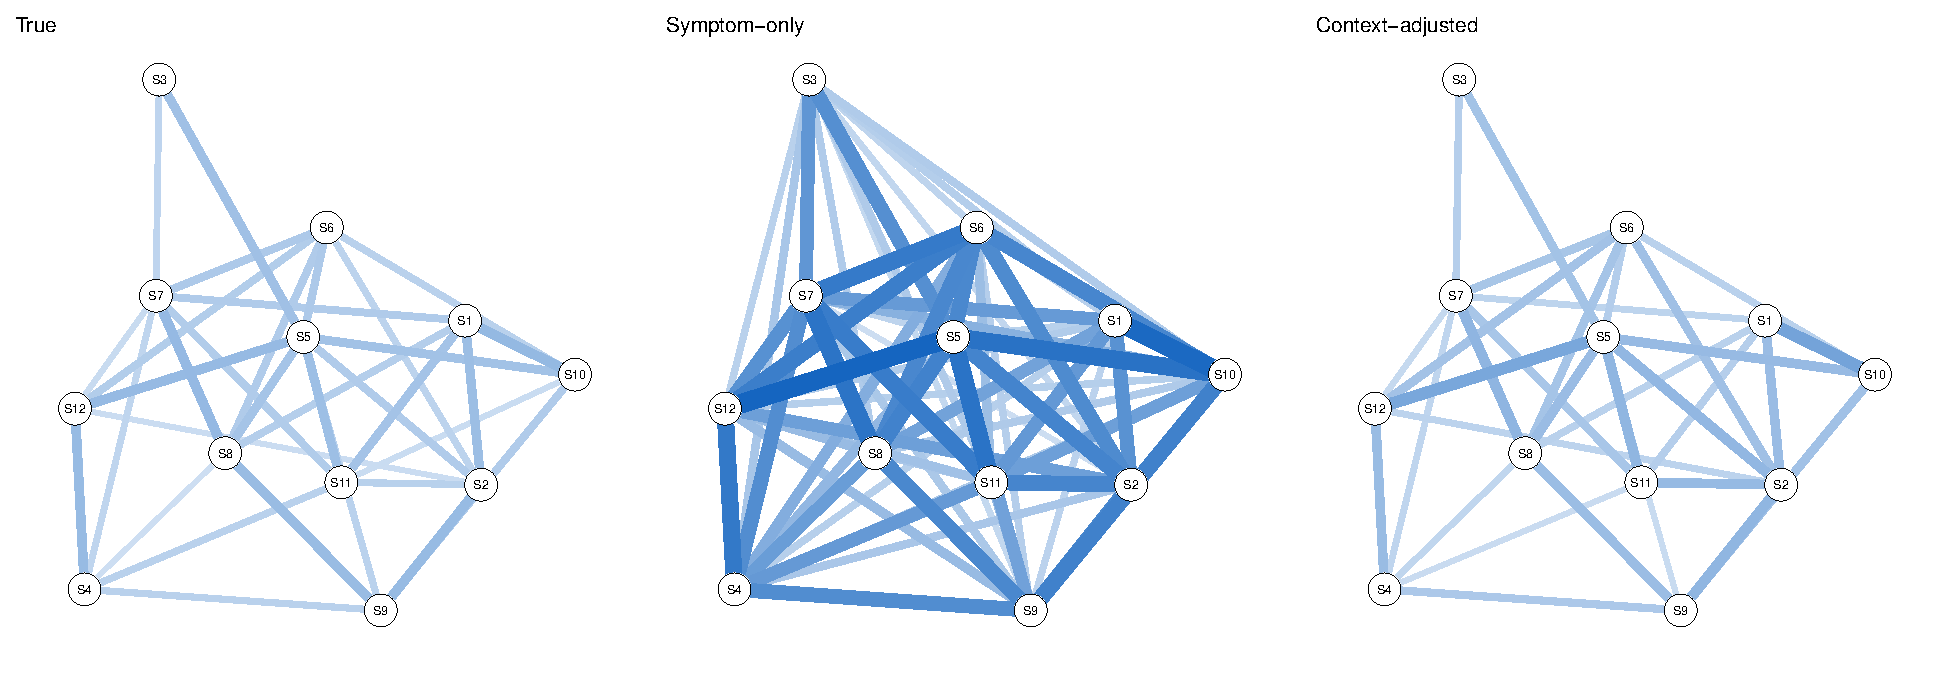
\includegraphics[width=\linewidth]{figs/Figure8_network_estimation_check_graphs.pdf}
  \caption{\textbf{Example estimated networks under omitted versus included slow context.} Networks
  were estimated from one representative data-generating network and group (high baseline) under
  the model's own coupled feedback dynamics, at the largest diffusion level and shortest
  observation window examined (\(\sigma_P=0.65\), \(W=1\)) -- the condition where omitted-context
  distortion is most pronounced. Left: true data-generating coupling matrix. Middle and right:
  symptom-only and context-adjusted estimates, averaged elementwise across 20 independent
  replicates of the same condition (matching the averaging used to compute Figure~\ref{fig:network_check})
  so that single-replicate sampling noise in individual edges is not mistaken for a systematic
  pattern. Edge color indicates the sign of the estimated coupling (blue = positive, red =
  negative); consistent with the true network, no negative edges survive averaging across
  replicates in either estimated panel. Edges below a common plotting
  threshold are omitted for clarity in the two estimated panels (the true panel is shown at full
  precision, since it has no sampling noise to threshold away), and the same spring layout, derived
  from the true network, and the same edge-weight scaling are used across all three panels. Omitting slow context yields a substantially denser network than the true structure, whereas
  including slow context recovers an estimate visibly closer to it.}
  \label{fig:network_check_graphs}
\end{figure}
% ==================================================================
% Discussion
% ==================================================================
\section{Discussion}
The starting point for this paper was a simple ambiguity in the interpretation of symptom networks. If two groups show different symptom-network patterns, it is tempting to conclude that their symptoms interact differently. Yet symptoms do not unfold in isolation. They arise within slower-moving social, relational, economic, and biological conditions that can make symptoms easier or harder to activate. In network terms, these conditions form part of the external field of the symptom system: they may not be symptoms themselves, but they change the conditions under which symptoms become active \parencite{borsboom2017network}. The present paper formalized this ambiguity in a slow--fast model. The fast layer captured symptom activation under fixed symptom--symptom coupling, while the slow layer shifted the threshold regime in which those symptoms became active.
The results show that slow threshold shifts can generate several qualitatively different between-group patterns without changing the fast-layer interaction structure. When the fast layer is monostable, group differences in the slow-state baseline produce stable separation in symptom levels, but not abrupt regime change. When the fast layer is bistable-capable, the same kind of baseline difference can place one group closer to a transition boundary, so that gradual drift and symptom-to-slow-state feedback can produce abrupt and persistent shifts into a high-symptom state. When acute stressors are added, their consequences depend on this regime structure. In the monostable case, stressors mainly produce temporary worsening. Near a transition boundary, however, a similar perturbation can move the system into a persistent high-symptom state. Thus, the central result is not merely that threshold shifts can matter, but that their consequences depend on where the system is located in the slow--fast equilibrium structure.
This result connects to, but also extends, existing work on network dynamics in psychopathology. Previous theoretical and simulation work has shown how feedback among symptoms can produce self-sustaining symptom activation, alternative stable states, and hysteresis-like dynamics \parencite{borsboom2017network, cramer2016major, van2014critical}. Critical-transition approaches have further emphasized that nonlinear psychological systems may show tipping points, slowing recovery, and early warning signals as they approach transitions \parencite{scheffer2009early, van2014critical, helmich2021early}. The present model keeps this dynamic intuition, but shifts the focus from symptom--symptom coupling alone to the interaction between coupling and threshold regime. In doing so, it clarifies why the same level of symptom--symptom coupling can have different consequences depending on the slower conditions in which the symptom system is embedded.
The main implication is interpretive. Large differences in symptom levels, symptom trajectories, or estimated psychological networks do not by themselves imply differences in symptom--symptom coupling. In the present framework, the same fast-layer parameters can produce substantially different outcomes because groups differ in the baseline level, variability, feedback, or acute-stressor exposure of the slow state. A group may appear more symptomatic, more unstable, or more likely to occupy a high-symptom state not because its symptom interactions are stronger or differently organized, but because its slow-state conditions make symptoms easier to activate or place the system closer to a transition boundary. This is especially important for cross-sectional group comparisons, where the observed symptom pattern provides limited information about whether a group difference arose from coupling, thresholds, recent perturbations, or proximity to a transition.
The substantive interpretation changes accordingly. A coupling-based account suggests that groups differ in the mechanisms by which symptoms reinforce one another. This may motivate symptom-focused or edge-focused explanations, such as targeting central symptoms or changing particular symptom--symptom relations. A threshold-shift account points to a different possibility: the relevant difference may lie in the background conditions that shift activation thresholds. In that case, the clinical target is not only the symptom system itself, but also the slower processes that make symptom activation more likely, more stable, or more difficult to escape. For example, if a group difference is driven by contextual conditions that keep symptoms close to a transition boundary, then interventions aimed only at symptom interactions may miss part of the mechanism. Interventions that reduce chronic stress exposure, increase social support, improve sleep and recovery, reduce financial pressure, or address relevant biological conditions may shift the system away from the boundary and thereby change how the same symptom network behaves.
This distinction also matters for how group comparisons are evaluated methodologically. Network-comparison and moderation approaches provide valuable tools for asking whether estimated thresholds or interactions differ across groups \parencite{van2023comparing, haslbeck2022estimating}. However, the present model highlights a generative question that comes before interpretation: what data-generating process could have produced the observed group difference? A difference in estimated connectivity may reflect true differences in interaction parameters, but it may also reflect differences in threshold regimes, slow covariates, sampling from different regions of a nonlinear response surface, or unmodeled contextual processes. This does not mean that between-group network comparisons are uninformative. Rather, it means that they should be interpreted together with threshold parameters, relevant slow covariates, longitudinal information, and sensitivity analyses that ask whether similar patterns could arise under fixed coupling.
The network-estimation check made this identification problem concrete. When the slow context was omitted, data generated from the same coupling matrix produced increasingly inflated estimates of global strength as slow-context variation increased. Including the slow context largely removed this inflation and improved recovery of the true coupling matrix. This result does not imply that all empirical group differences in symptom networks are artifacts of omitted context. Rather, it shows that estimated connectivity can contain contributions from unmodeled slow contextual variation. In such cases, stronger estimated symptom--symptom coupling may partly reflect shared exposure to, or movement along, a slower contextual process rather than stronger direct coupling among symptoms themselves.
The model also speaks to a broader issue in psychological theory. Many psychological processes involve fast-changing states embedded in slower-changing conditions. Affect, motivation, attention, executive control, interpersonal behavior, and symptoms can fluctuate over short timescales, while stress exposure, social support, financial insecurity, sleep and fatigue, inflammation, hormonal regulation, and other contextual or biological processes often change more gradually. Experience-sampling and dynamic-network approaches have made major progress in studying short-term psychological fluctuations \parencite{myin2009experience, wichers2014dynamic, bringmann2013network}. Other lines of work have emphasized slower processes such as personality, resilience, vulnerability, and stress generation \parencite{lunansky2020personality, hammen2006stress, liu2010stress, rnic2023vicious}. Slow--fast modeling provides a way to connect these levels. It asks how slower conditions shape the ease with which fast psychological states become active, and how sustained fast-state activation can, over time, reshape the slower conditions that maintain the system.
This perspective may be especially useful for understanding why similar events have different consequences for different people or groups. A conflict, financial setback, poor night of sleep, or health problem may produce only transient symptom elevation in one context, but trigger a persistent episode in another. In the model, this difference does not require the acute event itself to be qualitatively different. It can arise because the slow state has already moved the system closer to a transition boundary. This provides a formal way to express a familiar clinical idea: the effect of a stressor depends not only on the stressor, but also on the state of the person and the conditions in which the stressor occurs. The same perturbation may dissipate in a resilient regime and persist in a vulnerable one.
The framework is intentionally minimal. The mean-field fast layer provides analytic clarity, but it compresses symptom heterogeneity into a homogeneous interaction structure and a single summary variable. Real symptom systems are likely to contain symptom-specific thresholds, heterogeneous coupling patterns, and subgroups of symptoms that interact more strongly with one another than with the rest of the system. The slow state is also represented as a single dimension, whereas real clinical systems are shaped by multiple interacting slow processes, including social, financial, relational, biological, and developmental influences. Finally, acute stressors are modeled as discrete perturbations to the slow state generated by a simple baseline and symptom-linked hazard process, rather than as a full model of how stressful events arise, vary in severity, or depend on context \parencite{hammen2006stress,dohrenwend2006inventorying,cohen2019ten}. Future work could examine more directly whether episodes that emerge gradually from accumulating strain differ from episodes triggered by sudden events, for example in how predictable they are from earlier symptom patterns.
These simplifications are also what make the model useful as a first step. By holding symptom--symptom coupling fixed across groups, the simulations isolate what slow threshold shifts alone can do. Future work can relax these assumptions by allowing symptom-specific thresholds \(h_i(P)\), heterogeneous or modular coupling structures, multiple slow variables, empirically grounded mappings from measured covariates to \(P(t)\), and richer models of acute stressor exposure. Such extensions would make it possible to ask, in more realistic settings, how much of an observed group difference is attributable to coupling, how much to threshold shifts, and how much to the interaction between fast symptom dynamics and slower contextual conditions.
In sum, the model reframes between-group differences in symptom networks as a problem of interacting timescales. Symptoms may reinforce one another, but whether that reinforcement produces stable low-symptom states, temporary worsening, abrupt tipping, or persistent high-symptom states depends on the slower conditions in which the symptom system is embedded. Slow--fast coupling therefore provides a general framework for studying psychological systems in which fast-changing states are shaped by slower-moving conditions, and in which those fast states can, over time, reshape the conditions that sustain them.
\printbibliography
% ===========================================================
% Appendix: Hysteresis protocol
% ===========================================================
\appendix
\section{Technical details of the model}
This appendix provides technical details that complement the streamlined model description in the main text. The main text focuses on the conceptual structure of the slow--fast system and the key equations needed to interpret the simulations. Here we collect the update-level derivations and implementation details for the fast layer, the slow memory term, and the shock process.
\subsection{Fast-layer update dynamics}
In simulations, the fast layer is updated by repeated Monte Carlo sweeps within each slow time step, while the slow state is held fixed. One sweep consists of \(N\) random single-site updates with replacement. In the simulations reported in the main text, we use 40 sweeps per slow time step. The mean-field input is recomputed once per sweep and then held constant during the \(N\) single-site updates within that sweep, corresponding to a sweep-level mean-field approximation.
To characterize the implied dynamics of the mean symptom level \(m\), consider a single asynchronous update. One symptom is chosen uniformly at random. Because \(m\) is the fraction of active symptoms, it can change only in steps of size \(1/N\): it increases by \(1/N\) if an inactive symptom is selected and switches to active, and it decreases by \(1/N\) if an active symptom is selected and switches to inactive.
Let
\[
p(m,p_t)=\sigma\!\big(\beta H(m,p_t)\big)
\]
denote the probability that a selected symptom is active after update, given the current mean symptom level \(m\) and slow state \(p_t\). The probability of selecting an inactive symptom is \(1-m\), and the probability of selecting an active symptom is \(m\). Therefore,
\[
\Pr\!\left(m\to m+\frac{1}{N}\,\middle|\,m,p_t\right)=(1-m)\,p(m,p_t),
\]
and
\[
\Pr\!\left(m\to m-\frac{1}{N}\,\middle|\,m,p_t\right)=m\,\bigl(1-p(m,p_t)\bigr).
\]
Taking expectations gives
\[
\mathbb{E}[\Delta m\mid m,p_t]
=\frac{1}{N}\bigl(p(m,p_t)-m\bigr).
\]
Thus, the dynamics of \(m\) can be viewed as a biased random walk on \([0,1]\): on average, the mean symptom level is pulled toward \(p(m,p_t)\), the probability that a selected symptom is active after update. Writing \(F(m;p_t)=p(m,p_t)\), equilibrium values of the fast layer satisfy
\[
m = F(m;p_t).
\]
\subsection{Local stability and the bistability threshold}
For a fixed slow state \(P\), equilibria of the fast layer are fixed points of the mean-field response function \(F(m;P)\), that is, values \(m^\ast\) satisfying
\[
m^\ast = F(m^\ast;P).
\]
To determine whether a fixed point attracts nearby states, consider a small perturbation \(m_t=m^\ast+\varepsilon_t\) with \(|\varepsilon_t|\ll 1\). A first-order Taylor expansion of \(F\) around \(m^\ast\) gives
\[
m_{t+1}=F(m^\ast+\varepsilon_t;P)\approx F(m^\ast;P)+F'(m^\ast;P)\,\varepsilon_t
= m^\ast + F'(m^\ast;P)\,\varepsilon_t,
\]
where we used \(F(m^\ast;P)=m^\ast\). Hence
\[
\varepsilon_{t+1}\approx F'(m^\ast;P)\,\varepsilon_t.
\]
A fixed point is therefore locally stable if nearby perturbations shrink,
\begin{equation}\label{eq:stability}
|F'(m^\ast;P)|<1,
\end{equation}
and unstable if \(|F'(m^\ast;P)|>1\). Since \(F\) increases in \(m\) for \(J>0\), this reduces to \(F'(m^\ast;P)<1\).
For the present model,
\[
F(m;P)=\sigma\!\left(\beta\left[J\left(m-\tfrac12\right)+h+\gamma P\right]\right).
\]
Let
\[
z=\beta\left[J\left(m-\tfrac12\right)+h+\gamma P\right].
\]
Using \(\sigma'(z)=\sigma(z)\bigl(1-\sigma(z)\bigr)\) and \(\frac{dz}{dm}=\beta J\), the chain rule gives
\begin{equation}\label{eq:Fprime}
F'(m;P)=\beta J\,\sigma(z)\bigl(1-\sigma(z)\bigr).
\end{equation}
Because \(\sigma(z)\bigl(1-\sigma(z)\bigr)\le \tfrac14\), with equality at \(\sigma(z)=\tfrac12\), the slope is bounded by
\[
F'(m;P)\le \frac{\beta J}{4}.
\]
This yields the bistability threshold. If \(\beta J\le 4\), the update curve can never become steeper than the diagonal, so for generic parameter values there is a single equilibrium for each \(P\). If \(\beta J>4\), the curve can become locally steeper than the diagonal near its inflection region, allowing three intersections over an intermediate range of \(P\): two stable outer equilibria separated by one unstable middle equilibrium.
\subsection{Slow memory and shock implementation}
\subsubsection{Smoothed symptom signal}
The slow state depends not on the instantaneous symptom level \(m_t\), but on the exponentially weighted moving average
\[
m_{\text{slow},t+dt} = (1-\lambda_m)\,m_{\text{slow},t} + \lambda_m\,m_t,
\qquad 0<\lambda_m<1.
\]
Equivalently,
\[
m_{\text{slow},t+dt}=m_{\text{slow},t}+\lambda_m\big(m_t-m_{\text{slow},t}\big).
\]
Thus, \(m_{\text{slow},t}\) moves only partway toward the current \(m_t\) at each step.
Iterating this recursion yields
\[
m_{\text{slow},t}
=
\lambda_m\sum_{k=0}^{t-1}(1-\lambda_m)^k\,m_{t-1-k}
+
(1-\lambda_m)^t m_{\text{slow},0}.
\]
This shows that past values receive geometrically decaying weights: observations \(k\) steps in the past are weighted proportionally to \((1-\lambda_m)^k\). Smaller \(\lambda_m\) therefore implies longer memory and stronger separation between the fast and slow timescales.
\subsubsection{Shock process}
Rare acute events are represented as additive shock increments \(\xi_t\) in the slow-state update.
Conceptually, the shock term is meant to capture discrete, identifiable events with their own
timing and effect size, such as a relationship change, bereavement, job loss, financial setback,
or health problem. This differs from the Gaussian diffusion term in Eq.~\eqref{eq:slow_update},
which represents the accumulation of many smaller, unidentified background influences whose
individual timing and magnitude are not distinguished.
We assume that shocks occur as rare Poisson events with instantaneous rate
\begin{equation}
\lambda_{\text{tot}}(t)
=
\lambda_0
+
\lambda_1\,\big[m_{\text{slow},t}-m_{\text{crit}}\big]_+,
\qquad [x]_+\equiv \max(0,x),\quad \lambda_1\ge 0.
\label{eq:lambda_tot_app}
\end{equation}
Here, \(\lambda_0\) is a baseline event rate and \(\lambda_1\) controls the additional event risk when the smoothed symptom signal exceeds the threshold \(m_{\text{crit}}\).
To simulate this process on a time grid of size \(dt\), we convert the continuous-time event rate into the probability that at least one event occurs during the next step:
\[
p_{\text{tot}}(t)=1-\exp\!\big(-\lambda_{\text{tot}}(t)\,dt\big),
\qquad
I_t\sim\mathrm{Bernoulli}\!\big(p_{\text{tot}}(t)\big).
\]
We interpret \(I_t=1\) as an event occurring during \([t,t+dt)\), and \(I_t=0\) as no event. For sufficiently small \(dt\), this approximation allows at most one event per step while keeping the probability of multiple events within a single step negligible.
This construction also clarifies why \(\xi_t\) is added directly to the slow-state update rather
than multiplied by \(dt\). In the discrete-time approximation, the probability of a jump occurring
during a step scales with \(dt\), through \(p_{\text{tot}}(t)\), but the jump size itself does not.
Thus, as the time grid is refined, diffusion increments become smaller per step, whereas a realized
shock remains a finite displacement of the slow state. This is what distinguishes an acute event
from the continuous accumulation of smaller background fluctuations.
Conditional on \(I_t=1\), we label the event as symptom-triggered versus baseline in proportion to their contributions to the total rate:
\[
\Pr(\text{triggered}\mid I_t=1)=
\frac{\lambda_1[m_{\text{slow},t}-m_{\text{crit}}]_+}{\lambda_{\text{tot}}(t)},
\qquad
\Pr(\text{baseline}\mid I_t=1)=\frac{\lambda_0}{\lambda_{\text{tot}}(t)}.
\]
We then draw an event-type-specific magnitude and set the shock increment for that step:
\[
\xi_t=
\begin{cases}
A_{\text{base},t}, & \text{baseline event},\\
A_{\text{trig},t}, & \text{symptom-triggered event},\\
0, & I_t=0,
\end{cases}
\qquad
A_{\text{base},t}\sim \mathcal{N}(\mu_{\text{base}},\sigma^2_{\text{base}}),\quad
A_{\text{trig},t}\sim \mathcal{N}(\mu_{\text{trig}},\sigma^2_{\text{trig}}).
\]
\section{Hysteresis under an exogenous slow-state ramp (diagnostic)}\label{sec:appendix_hysteresis}
This appendix shows the hysteresis pattern of the model in a cleaner setting. Instead of using the full slow dynamics from the main simulations, we impose a baseline context \(P_{\text{base}}(t)\) that slowly increases from a low value to a high value and then returns to its starting level ("ramp reversal"), while turning off symptom-to-context feedback by setting \(b=0\) in Eq.~\eqref{eq:slow_update}. The slow state \(P_t\) is then simulated using this changing baseline and the usual context update. In this setting, \(P_t\) tracks the imposed baseline with some lag due to mean reversion and diffusion noise. This lets us see the basic path-dependent structure of the fast layer more clearly: when \(\beta J>4\), the same value of the slow state \(P\) can correspond to different symptom levels depending on whether the system is approached from lower or higher values.
Figure~\ref{fig:hysteresis} shows the characteristic hysteresis pattern of the model. Panel~A compares the imposed slow-state ramp \(P_{\text{base}}(t)\) (dashed) with the realized context \(P_t\) (solid), showing that the slow state tracks the external ramp with some lag. Panel~B shows the corresponding symptom trajectory \(m_t\): as \(P_t\) is driven upward and then downward, the symptom level does not change smoothly throughout, but instead undergoes abrupt jumps between low- and high-symptom branches. The dashed vertical lines mark these transition times. Panel~C makes the path dependence explicit by plotting \(m_t\) against \(P_t\). During the upward and downward phases of the ramp, the system follows different branches, so the same value of the slow state can correspond to different symptom levels depending on the direction from which it is approached.
This diagnostic helps interpret the regime maps in the main text by showing how relatively small changes in context can trigger abrupt transitions between low- and high-symptom states when the system operates near the bistable region.
\begin{figure}[htbp]
  \centering
  \makebox[\textwidth][c]{%
  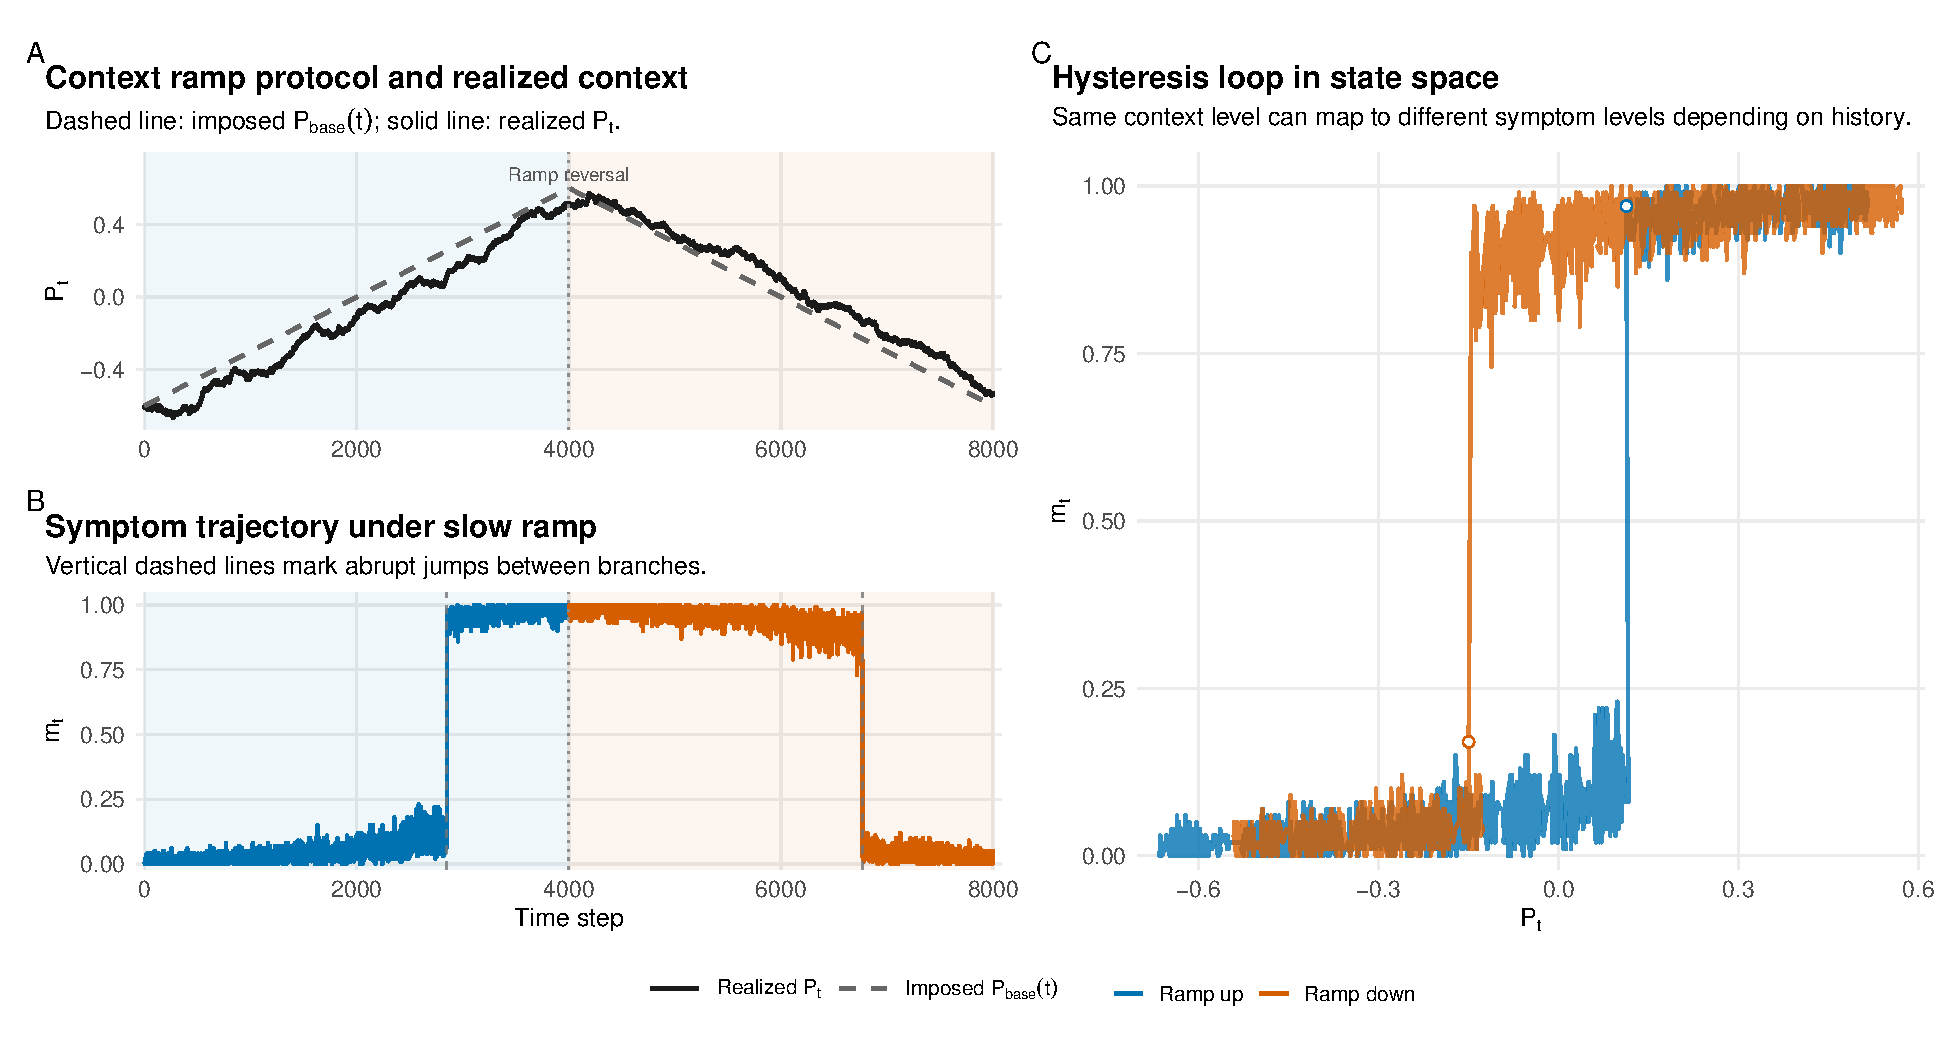
\includegraphics[width=1.15\linewidth]{figs/Figure_hysteresis.pdf}}
\caption{\textbf{Hysteresis under a slow exogenous slow-state ramp.}
The fast layer is bistable-capable (\(\beta J>4\)) and the symptom-to-context feedback term is turned off by setting \(b=0\) in Eq.~\eqref{eq:slow_update}. \textbf{(A)} The imposed baseline context \(P_{\text{base}}(t)\) (dashed) is slowly increased and then decreased; the realized slow state \(P_t\) (solid) follows this ramp with slight lag. \textbf{(B)} The corresponding mean symptom level \(m_t\) does not vary smoothly throughout the ramp, but instead shows abrupt jumps between low- and high-symptom branches as \(P_t\) crosses fold boundaries; vertical dashed lines mark these transition times. \textbf{(C)} Plotting \(m_t\) against \(P_t\) reveals a hysteresis loop: during the upward and downward phases of the ramp, the system follows different branches, so the same value of the slow state can correspond to different symptom levels depending on history.}
  \label{fig:hysteresis}
\end{figure}
\section{Network-estimation check: implementation details}\label{app:network_check_details}
This appendix reports the full implementation details for the network-estimation check
summarized in Section~\ref{sec:network_estimation_check} and Section~\ref{sec:res_network_check}.
Each simulated individual ran their own private coupled fast/slow system, in which sustained
symptom elevation (via the smoothed signal \(m_{\text{slow}}\), Eq.~\eqref{eq:mslow}) fed back
onto their own \(P_t\) through the calibrated slow-state equation (Eq.~\eqref{eq:slow_update}). We
swept two design factors that jointly determine how much of this coupled process an observer sees.
First, the model's own diffusion parameter \(\sigma_P\) was swept across four levels,
\(\sigma_P\in\{0.04,0.15,0.35,0.65\}\): the lowest is the calibrated value used throughout the
rest of the paper (Table~\ref{tab:scenario_design}), and the highest was chosen so that the
resulting between-person spread at the shortest window matches the upper end of the range this
check swept directly in an earlier, exogenous design. Second, the length of the observation window
\(W\) used to construct each measurement was swept from a single near-instantaneous snapshot
(\(W=1\) step) to long temporal aggregation (\(W=5{,}000\) steps, \(W/\tau_P=20\), where
\(\tau_P=1/\kappa\) is the context's own relaxation time). For a given \(\sigma_P\) and \(W\), each
individual's context covariate was the window average
\(\bar P_W=\frac{1}{W}\sum_{t=\text{burn-in}+1}^{\text{burn-in}+W}P_t\), computed after a
3{,}000-step burn-in verified sufficient for the coupled dynamics to reach a stable regime; their
single observed symptom vector was drawn conditional on \(\bar P_W\) rather than on the
instantaneous context at any one step, operationalizing ``an observation aggregated over window
\(W\).''
We implemented this check with \(N=12\) symptoms, matching the network size used in the
supplementary NCT check (Appendix~\ref{app:nct}). \(W^{\mathrm{true}}\) had edge density 0.5, with
nonzero weights drawn from \(\mathrm{Uniform}(0.15,0.35)\); thresholds \(h_i\) and slow-context
loadings \(\gamma_i\) were drawn from \(\mathrm{Uniform}(-1.6,-1.0)\) and \(\mathrm{Uniform}(0.8,1.4)\),
respectively. Groups differed only in the baseline level their context was pulled toward (low
baseline: \(P_{\text{base}}=-0.3\); high baseline: \(P_{\text{base}}=1.0\)), with feedback
(\(b=0.15\)) and all other slow-state parameters fixed at their calibrated values
(\(\kappa=0.20\), \(\lambda_m=0.001\), \(m_\star=0.25\); Table~\ref{tab:scenario_design}) throughout
-- feedback was never disabled, and \(\sigma_P\) was the only parameter varied away from its
calibrated value. To avoid results specific to one arbitrary network, we repeated the full
\(\sigma_P\times W\) design (16 combinations) across 3 independently drawn data-generating
networks and 3 replicates per network, with 1{,}000 individuals per group per replicate, and
estimated networks via nodewise logistic regression, symmetrized by averaging directed
coefficients.
\section{Supplementary check: NCT under threshold differences only}\label{app:nct}
To examine whether standard network comparison procedures absorb threshold differences into threshold parameters rather than into edge estimates, we conducted a supplementary Monte Carlo analysis. In each condition, we simulated two groups from Ising models with the same coupling matrix \(J\) but different threshold vectors, estimated the networks separately with \texttt{IsingFit}, and compared them using the weighted Network Comparison Test (NCT). Thus, the two groups were generated from the same underlying symptom network and differed only in their baseline tendency for symptoms to become active.
Table~\ref{tab:nct_design} summarizes the simulation design. The true network topology was varied across three cases: dense, modular, and ring. These are not participant groups, but three different coupling structures used to generate the data. Within each condition, both groups shared the same coupling matrix and differed only in thresholds.
\begin{table}[htbp]
\centering
\begin{threeparttable}
\caption{Design of the supplementary NCT simulation.}
\label{tab:nct_design}
\footnotesize
\setlength{\tabcolsep}{6pt}
\renewcommand{\arraystretch}{1.15}
\begin{tabularx}{\linewidth}{@{} l X @{}}
\toprule
\textbf{Category} & \textbf{Setting} \\
\midrule
Symptoms & \(N=12\) binary symptoms. \\
Groups & Two groups per replicate. The groups had identical coupling and differed only in thresholds. \\
Dense topology & Fully connected 12-node network: all off-diagonal edge weights set to \(0.25\), diagonal entries set to \(0\). \\
Modular topology & Two 6-node modules: all within-module off-diagonal edge weights set to \(0.25\), all between-module edge weights set to \(0.05\), diagonal entries set to \(0\). \\
Ring topology & 12-node ring: each node connected only to its two immediate neighbors with edge weight \(0.25\); all other off-diagonal entries set to \(0\). \\
Low-threshold group & All 12 thresholds set to \(-2.0\). \\
High-threshold group & All 12 thresholds set to \(-2.0+\Delta\), where \(\Delta \in \{0.4, 0.8, 1.2\}\). Thus the second group used thresholds \(-1.6\), \(-1.2\), or \(-0.8\). \\
Meaning of threshold difference & Less negative thresholds imply a higher baseline probability that symptoms are active. \\
Sample size per group & \(n \in \{200, 500, 1000\}\). \\
Monte Carlo replicates & 100 replicates per condition. \\
Data generation & \texttt{IsingSampler}, binary responses \(\{0,1\}\), Metropolis--Hastings sampler. \\
Network estimation & \texttt{IsingFit} with \texttt{family = "binomial"}. \\
Network comparison & Weighted \texttt{NCT}. \\
Permutations per NCT run & 250. \\
\bottomrule
\end{tabularx}
\end{threeparttable}
\end{table}
We summarized the results in three ways, shown in Table~\ref{tab:nct_outcomes}. First, we recorded how often NCT rejected the \emph{structure invariance test}, that is, how often it concluded that the estimated edge-weight configuration differed between the two groups. Second, we recorded how often NCT rejected the \emph{global strength test}, that is, how often it concluded that the total connectivity differed between groups. Third, because we requested edge-wise tests, we computed the average proportion of individual edges that were falsely flagged as significant at \(p<.05\). Under the null hypothesis of identical coupling, all three quantities would ideally remain close to the nominal \(5\%\) level.
\begin{table}[htbp]
\centering
\begin{threeparttable}
\caption{How the three supplementary NCT outcomes were measured.}
\label{tab:nct_outcomes}
\footnotesize
\setlength{\tabcolsep}{6pt}
\renewcommand{\arraystretch}{1.15}
\begin{tabularx}{\linewidth}{@{} l X @{}}
\toprule
\textbf{Outcome} & \textbf{Definition} \\
\midrule
Structure invariance rejection rate & Across the 100 replicates in a condition, the proportion for which the NCT structure test returned \(p<.05\). \\
Global strength rejection rate & Across the 100 replicates in a condition, the proportion for which the NCT global-strength test returned \(p<.05\). \\
Edge-level false-positive rate & For each replicate, the proportion of individual edge comparisons with \(p<.05\); the plotted value is the average of that proportion across replicates. \\
\bottomrule
\end{tabularx}
\end{threeparttable}
\end{table}
The results were mixed. The structure invariance test remained broadly close to the nominal \(5\%\) level, and edge-level false-positive rates were low overall. By contrast, the global strength test showed stronger inflation in dense networks, especially at the largest sample size. Thus, this supplementary analysis suggests that threshold differences do not necessarily create broad false evidence of different network structure, but they can still generate misleading differences in estimated global strength.
\begin{figure}[htbp]
  \centering
  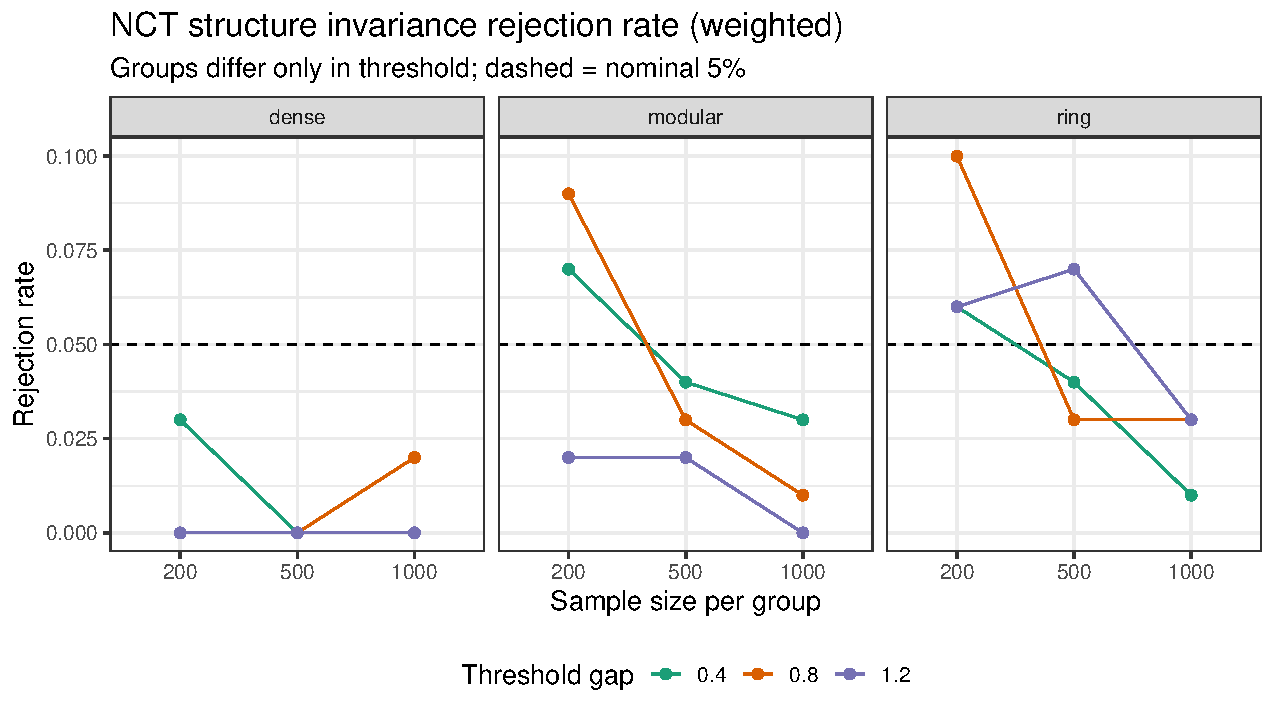
\includegraphics[width=\linewidth]{figs/nct_structure_weighted.pdf}
  \vspace{0.8em}
  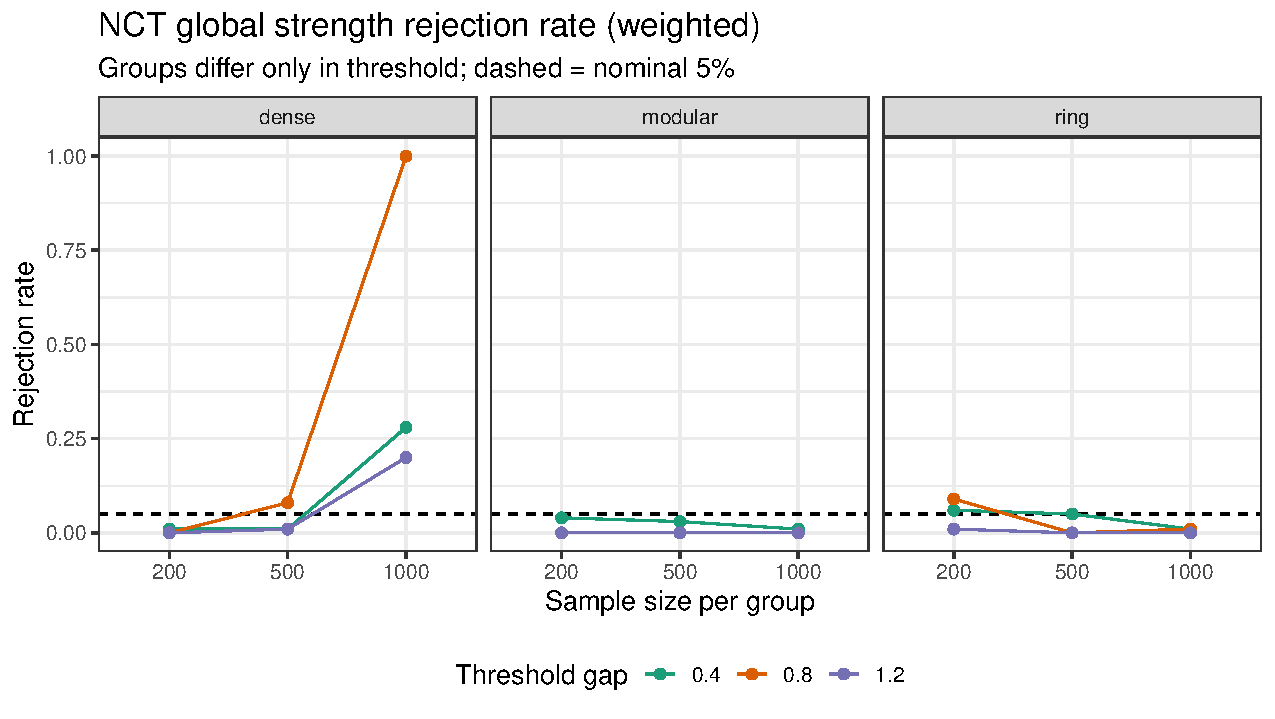
\includegraphics[width=\linewidth]{figs/nct_strength_weighted.pdf}
  \caption{\textbf{Supplementary Monte Carlo check of NCT under threshold differences only (Part 1).}
  Two groups were simulated with identical coupling but different thresholds and compared using weighted NCT. The dashed horizontal line marks the nominal \(5\%\) level under the null hypothesis that the two groups have the same coupling. Shown here are rejection rates for the structure invariance test and the global strength test.}
  \label{fig:appendix_nct_part1}
\end{figure}
\begin{figure}[htbp]
  \centering
  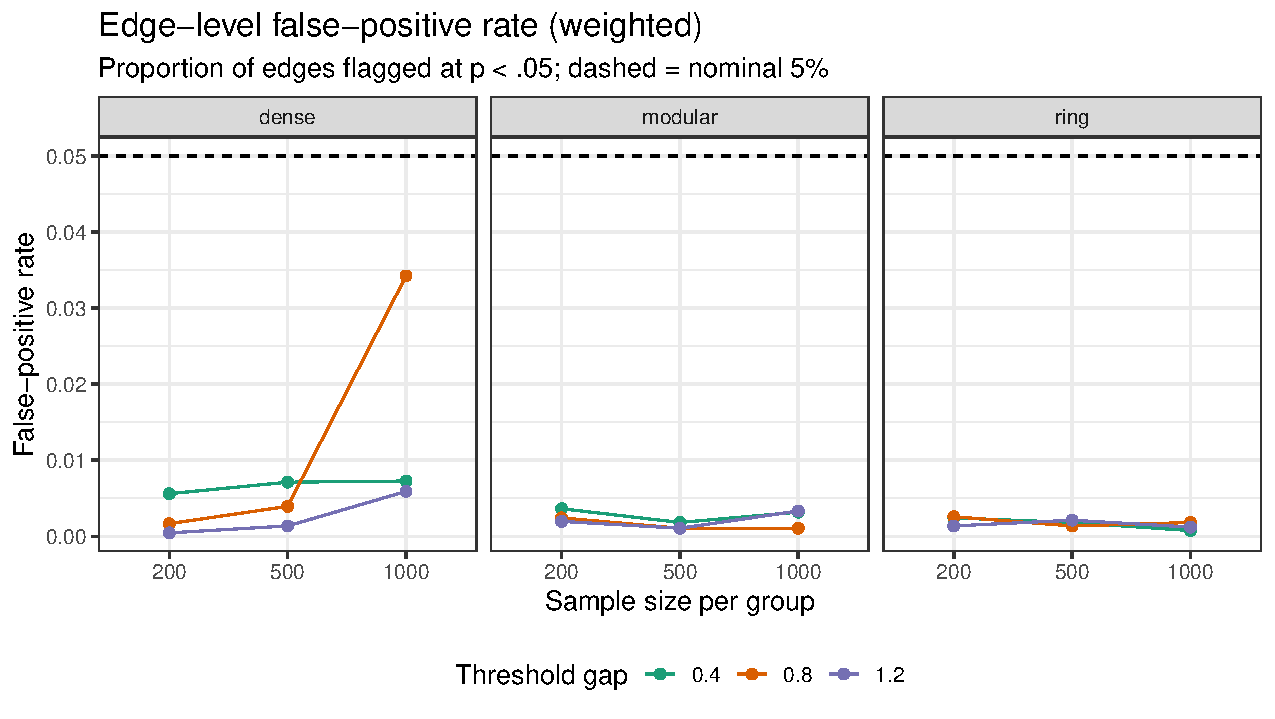
\includegraphics[width=\linewidth]{figs/nct_edge_fp_weighted.pdf}
  \caption{\textbf{Supplementary Monte Carlo check of NCT under threshold differences only (Part 2).}
  Edge-level false-positive rates from the same simulation. The dashed horizontal line marks the nominal \(5\%\) level. False-positive rates remained low overall.}
  \label{fig:appendix_nct_part2}
\end{figure}
\end{document}
%%
%% Copyright (C) 2019 by Daniel A. Weiss <daniel.weiss.led at gmail.com>
%%
%% This work may be distributed and/or modified under the
%% conditions of the LaTeX Project Public License (LPPL), either
%% version 1.3c of this license or (at your option) any later
%% version.  The latest version of this license is in the file:
%%
%% http://www.latex-project.org/lppl.txt
%%
%% Users may freely modify these files without permission, as long as the
%% copyright line and this statement are maintained intact.
%%
%% This work is not endorsed by, affiliated with, or probably even known
%% by, the American Psychological Association.
%%
%% This work is "maintained" (as per LPPL maintenance status) by
%% Daniel A. Weiss.
%%
%% This work consists of the file  apa7.dtx
%% and the derived files           apa7.ins,
%%                                  apa7.cls,
%%                                 apa7.pdf,
%%                                 README,
%%                                 APA7american.txt,
%%                                 APA7british.txt,
%%                                 APA7dutch.txt,
%%                                 APA7english.txt,
%%                                 APA7german.txt,
%%                                 APA7ngerman.txt,
%%                                 APA7greek.txt,
%%                                 APA7czech.txt,
%%                                 APA7turkish.txt,
%%                                 APA7endfloat.cfg,
%%                                 Figure1.pdf,
%%                                 shortsample.tex,
%%                                 longsample.tex, and
%%                                 bibliography.bib.
%%
%%
%%
%% This is file `./samples/shortsample.tex',
%% generated with the docstrip utility.
%%
%% The original source files were:
%%
%% apa7.dtx  (with options: `shortsample')
%% ----------------------------------------------------------------------
%%
%% apa7 - A LaTeX class for formatting documents in compliance with the
%% American Psychological Association's Publication Manual, 7th edition
%%
%% Copyright (C) 2019 by Daniel A. Weiss <daniel.weiss.led at gmail.com>
%%
%% This work may be distributed and/or modified under the
%% conditions of the LaTeX Project Public License (LPPL), either
%% version 1.3c of this license or (at your option) any later
%% version.  The latest version of this license is in the file:
%%
%% http://www.latex-project.org/lppl.txt
%%
%% Users may freely modify these files without permission, as long as the
%% copyright line and this statement are maintained intact.
%%
%% This work is not endorsed by, affiliated with, or probably even known
%% by, the American Psychological Association.
%%
%% ----------------------------------------------------------------------
